\chapter{Linear Algebra}
We will first review some of the main results of linear algebra that will be useful for 10.34. Then, we will move on to some of the applications of linear algebra to numerical methods, and how to numerically solve linear systems. Feel free to skip directly to \Cref{sec:complexity-of-matrix-and-vector-operations} if you are comfortable with the basics of linear algebra.

\section{Scalars, Vectors, and Matrices}
\subsection{Scalars}
\textbf{Scalars} are single numbers, which can be used to represent quantities, like mass, temperature, or time. In linear algebra, we typically work with scalars from a \textbf{field}, which is a set equipped with two operations (addition and multiplication). Commonly used field---the set of scalars--- include real numbers $ \mathbb{R} $ and complex numbers $ \mathbb{C} $.

The set of real numbers, commonly denoted by $ \mathbb{R} $, includes all rational and irrational numbers.
That is, it includes integers like $-1, 0, 1$, fractions like $ \frac{1}{2} $, and irrational numbers like $ \pi $ and $ \sqrt{2} $.

% The field $ \mathbb{C} $ is an extension of $ \mathbb{R} $ using the imaginary unit $ i $, defined by $ i^2 = -1 $.

\subsubsection*{Complex Numbers}
Complex numbers are the numbers that involves imaginary number.
Imaginary numbers can be constructed by using $i=\sqrt{-1}$ as a building block.
Whether this number actually exists or not is not important, but what’s important is we can \emph{conceptually define this number}, and with this definition, we can derive so many \emph{useful properties}.

Complex numbers are obtained by combining real numbers and imaginary numbers.
Conversely, any element in the set of complex number $\mathbb{C}$ can be expressed as the combination of real numbers and imaginary numbers, as follows:
\begin{equation*}
    z = a + b i, \quad a, b \in \mathbb{R}
\end{equation*}
We also often use the notation $ \operatorname{Re}(z) = a $ and $ \operatorname{Im}(z) = b $ to denote the real and imaginary parts of the complex number $ z $, respectively.

The \textbf{complex conjugate} of $ z $ is denoted by $\overline{z}$ and is defined as:
\begin{equation*}
  \overline{z} := a - b i
\end{equation*}
For real values, we have absolute values that represent the magnitude of the real number.
For complex numbers, we can also define a similar notion of magnitude by using the complex conjugate defined above.
The \textbf{magnitude} (or modulus) of $ z $ is
\begin{equation*}
  |z| := \sqrt{z \overline{z}}
\end{equation*}
The magnitude of a complex number $ z = a + bi $ can be conveniently computed as follows:
\begin{equation*}
  |z| = \sqrt{a^2 + b^2}.
\end{equation*}

\begin{exampleBox}
    \textbf{Example}: For $ z = 3 + 4i $, the conjugate is $ \overline{z} = 3 - 4i $, and the magnitude is $ |z| = \sqrt{3^2 + 4^2} = 5 $.
\end{exampleBox}

We can visualize complex numbers as points in the complex plane, with the real part on the horizontal axis and the imaginary part on the vertical axis (\autoref{fig:complex-plane}).

\begin{figure}[H]
  \centering
  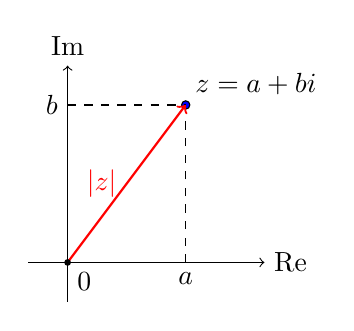
\begin{tikzpicture}[scale=.5]

    % Draw axes
    \draw[->] (-1, 0) -- (5, 0) node[right] {Re};
    \draw[->] (0, -1) -- (0, 5) node[above] {Im};

    % Define complex number
    \def\a{3}       % Real part
    \def\b{4}       % Imaginary part

    % Plot the complex number
    \draw[fill=blue] (\a, \b) circle[radius=3pt] node[above right] {$z = a + b i$};
    \node at (0, 4) [left] {$b$};
    \node at (3, 0) [below] {$a$};

    % Draw the vertical line to the real axis
    \draw[dashed] (\a, 0) -- (\a, \b);
    \draw[dashed] (0, \b) -- (\a, \b);

    % Draw the magnitude
    \draw[->, thick, red] (0, 0) -- (\a, \b) node[midway, left] {$|z|$};

    % Origin
    \draw[fill=black] (0, 0) circle[radius=2pt] node[below right] {0};
    
  \end{tikzpicture}
  \caption{The complex plane.}
    \label{fig:complex-plane}
\end{figure}

\subsection{Vectors}
A \textbf{vector} is a tuple---an ordered list---of scalars; it has magnitude and direction. In $ n $-dimensional space, a vector $ \mathbf{v} $ over the field $ \mathbb{R} $ or $ \mathbb{C} $ is written as
\begin{equation*}
    \mathbf{v} = (v_1, v_2, \ldots, v_n) = \begin{bmatrix} v_1 \\ v_2 \\ \vdots \\ v_n \end{bmatrix}, \quad v_i \in \mathbb{R} \text{ or } \mathbb{C}
\end{equation*}
It is common to write vectors either as tuples (arranged horizontally with comma separators) or as column vectors. We will use both notations interchangeably.
% SS: TODO: symbol (dimension for vector) is not consistent with the lecture notes. I like lowercase $n$ better, but for now, we should try to make the symbols consistent to reduce the confusion.

The set of $n$-dimensional vectors over the field $ \mathbb{R} $ is denoted by $ \mathbb{R}^n $, and the set of $n$-dimensional vectors over the field $ \mathbb{C} $ is denoted by $ \mathbb{C}^n $.
The set of all such vectors forms a \textbf{vector space} $ \mathbb{R}^n $ (or $ \mathbb{C}^n $).
Later in \Cref{sec:vector-space}, we will see that $\mathbb{R}^n$ and $\mathbb{C}^n$ form vector spaces, and several useful properties can be derived from the nature of vector spaces.

\subsubsection{Vector Operations}
\paragraph*{Vector Addition and Scalar Multiplication}
Two basic arithmetic operations can be defined over the vector space: \emph{addition} and \emph{scalar multiplication}.
Vector addition is defined for a pair of vectors with the same dimension.
Given two vectors $ \mathbf{u}, \mathbf{v} \in \mathbb{R}^n $ (or $ \mathbb{C}^n $), their addition is defined as follows:
\begin{equation*}
  \mathbf{u} + \mathbf{v} = \begin{bmatrix} u_1 + v_1 \\ u_2 + v_2 \\ \vdots \\ u_n + v_n \end{bmatrix}
\end{equation*}
That is, the addition is performed entry-wise.
This operation is commutative and associative. That is,
\begin{align*}
  \mathbf{u} + \mathbf{v} &= \mathbf{v} + \mathbf{u} \\
  (\mathbf{u} + \mathbf{v}) + \mathbf{w} &= \mathbf{u} + (\mathbf{v} + \mathbf{w}),
\end{align*}
for any vectors $ \mathbf{u}, \mathbf{v}, \mathbf{w} $ in the same vector space.
Geometrically, vector addition can be interpreted as a ``tip-to-tail'' construction (see \autoref{fig:vector-operations}).

\begin{warningBox}
  \textbf{Warning:} Vector addition is only defined for vectors of the same dimension. Attempting to add vectors of different dimensions is undefined. If you attempt to add vectors of different dimensions on a computer (e.g., in MATLAB), you will encounter an error:
\begin{verbatim}
>> [1; 2] + [3; 4; 5]
Arrays have incompatible sizes for this operation.
\end{verbatim}
\end{warningBox}

\paragraph*{Scalar Multiplication}
Scalar multiplication is defined for a vector and a scalar.
In particular, for a scalar $ c \in \mathbb{R} $ (or $ \mathbb{C} $) and a vector $ \mathbf{v}\in\mathbb{R}^{n} $ (or $\mathbb{C}^n$), the scalar multiplication is defined as follows:
\begin{equation*}
    c\mathbf{v} = \begin{bmatrix} c v_1 \\ c v_2 \\ \vdots \\ c v_n \end{bmatrix}
\end{equation*}
This operation is distributive over vector addition and scalar addition. That is,
\begin{align*}
  c(\mathbf{u} + \mathbf{v}) &= c\mathbf{u} + c\mathbf{v} \\
  (c + d)\mathbf{v} &= c\mathbf{v} + d\mathbf{v},
\end{align*}
for any vectors $ \mathbf{u}, \mathbf{v} $ in the same vector space and any scalars $ c, d $ in the same field.
Geometrically, scalar multiplication stretches or shrinks the vector by a factor of $ c $ (see \autoref{fig:vector-operations}).

\begin{figure}[H]
  \centering
  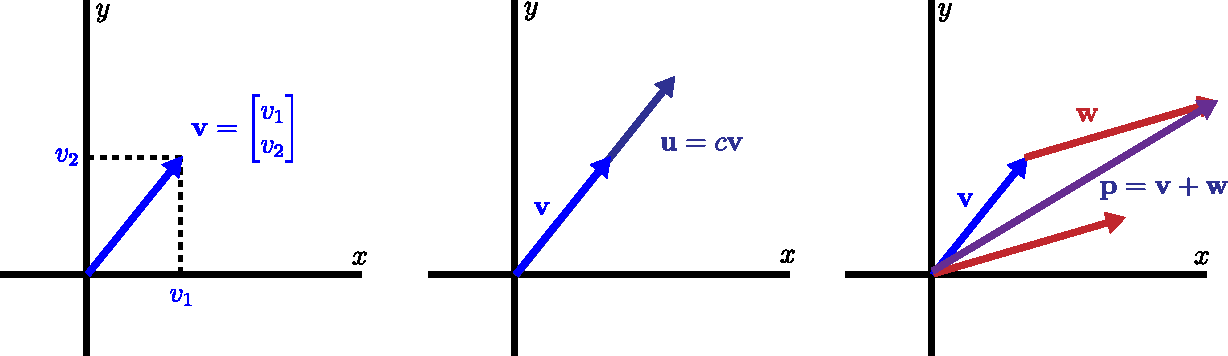
\includegraphics[width=0.85\textwidth]{figs/linear-algebra/vector-operations.pdf}
  \caption{Vector addition and scalar multiplication in $ \mathbb{R}^2 $.}
  \label{fig:vector-operations}
\end{figure}

You can also combine these two operations.
\begin{align}\label{eqn:ax+by}
  ax + by = \begin{bmatrix}
    a x_1 + b y_1 \\
    a x_2 + b y_2 \\
    \vdots \\
    a x_N + b y_N
  \end{bmatrix}
\end{align}
where $a$ and $b$ are scalar values, and $x$ and $y$ are vectors in $\mathbb{R}^N$.
We don't need to separetly define subtraction, since $x-y$ is equivalent to \cref{eqn:ax+by} with $a=1$ and $b=-1$.


We can observe that the result of scalar multiplication, vector addition, and even their combination is \emph{closed} within the vector space where $x$ and $y$ lives in.
This means that $ax + by$ is in $\mathbb{R}^N$, if $x$ and $y$ are in $\mathbb{R}^N$ and $a$ and $b$ are in $\mathbb{R}$.
The same goes true if you replace $\mathbb{R}$ with $\mathbb{C}$.
This observation is one of the key properties of vector spaces, and we will see more about vector spaces in \Cref{sec:vector-space}.

\emph{Null vector}, or zero vector, is a special vector whose all entries are zero:
\begin{align*}
  \boldsymbol{0} = (0, 0, \dots, 0).
\end{align*}


\subsection{Matrices}
A \textbf{matrix} is a rectangular array of scalars arranged in rows and columns. An $ m \times n $ matrix $ \mathbf{A} $ has $ m $ rows and $ n $ columns:
\begin{equation*}
    \mathbf{A} = \begin{bmatrix} 
        a_{11} & a_{12} & \ldots & a_{1n} \\ 
        a_{21} & a_{22} & \ldots & a_{2n} \\ 
        \vdots & \vdots & \ddots & \vdots \\ 
        a_{m1} & a_{m2} & \ldots & a_{mn} 
    \end{bmatrix}.
    % SS: notation inconsistent with the lecture slides. Fix later.
\end{equation*}
% Matrices can represent linear transformations from $ \mathbb{R}^n $ to $ \mathbb{R}^m $. % SS: later
The notation $ \mathbf{A} \in \mathbb{R}^{m \times n} $ indicates the dimensions of $ \mathbf{A} $ (and the fact that the entries are drawn from $\mathbb{R}$), and the notation $ a_{ij} $ denotes the element in the $ i $-th row and $ j $-th column.
Additionally, we can think of vectors as matrices with a single column---that is, as $ n \times 1 $ matrices.
This perspective allows us to treat vectors and matrices in a unified manner.

\subsubsection{Matrix Operations}

\paragraph*{Matrix Addition and Scalar Multiplication}
Like vectors, matrices can be added and scaled entry-wise:
\begin{itemize}
    \item \textbf{Addition}: $ (\mathbf{A} + \mathbf{B})_{ij} = a_{ij} + b_{ij} $
    \item \textbf{Scalar Multiplication}: $ (c\mathbf{A})_{ij} = c \cdot a_{ij} $
\end{itemize}

\paragraph*{Dot Product}
The \textbf{dot product} (inner product) of vectors $ \mathbf{u}, \mathbf{v} \in \mathbb{R}^n $ is
\begin{equation*}
    \mathbf{u}\cdot\mathbf{v} = \mathbf{u}^\top \mathbf{v} = \sum_{i=1}^n u_i v_i
\end{equation*}
It measures the projection of one vector onto another, which we can geometrically interpret as the product of the magnitudes of the vectors and the cosine of the angle between them (\autoref{fig:dot-product}). 

\begin{figure}[H]
    \centering
    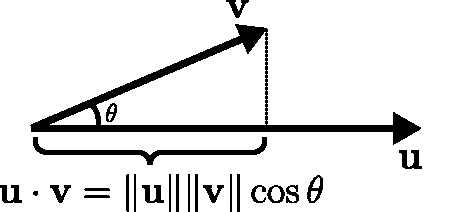
\includegraphics[width=0.35\textwidth]{figs/linear-algebra/dot-product.pdf}
    \caption{Geometric interpretation of the dot product.}
    \label{fig:dot-product}
\end{figure}

The dot product satisfies the following properties:
\begin{itemize}
    \item $ \mathbf{u} \cdot \mathbf{v} = \mathbf{v} \cdot \mathbf{u} $ (commutativity)
    \item $ \mathbf{u} \cdot (\mathbf{v} + \mathbf{w}) = \mathbf{u} \cdot \mathbf{v} + \mathbf{u} \cdot \mathbf{w} $ (distributivity)
    \item $ (\alpha \mathbf{u}) \cdot \mathbf{v} = \alpha (\mathbf{u} \cdot \mathbf{v}) $ (homogeneity)
    \item $ \mathbf{u} \cdot \mathbf{u} \geq 0 $ and $ \mathbf{u} \cdot \mathbf{u} = 0 $ if and only if $ \mathbf{u} = \mathbf{0} $ (positive definiteness)
\end{itemize}

\paragraph*{Matrix-Vector Products}
The product of an $m\times n$ matrix $ \mathbf{A} \in\mathbb{R}^{m\times n}$ and an $n$-dimensional vector $ \mathbf{x} $ is an $m$-dimensional vector $\mathbf{b}\in \mathbb{R}^m $:
\begin{equation*}
  b_i = \sum_{j=1}^n a_{ij} x_j.
\end{equation*}
Writing out everything explicitly, we have
\begin{equation*}
  \mathbf{b} = \mathbf{A}\mathbf{x} = \begin{bmatrix}
    a_{11}x_1 + a_{12}x_2 + \cdots + a_{1n}x_n \\
    a_{21}x_1 + a_{22}x_2 + \cdots + a_{2n}x_n \\
    \vdots \\
    a_{m1}x_1 + a_{m2}x_2 + \cdots + a_{mn}x_n
  \end{bmatrix}.
\end{equation*}

The number of columns in $ \mathbf{A} $ must equal the number of elements in $ \mathbf{x} $ for the product to be defined. Since vectors can be thought of as matrices with one column, matrix-vector multiplication is just a special case of matrix multiplication.

\begin{exampleBox}
  \textbf{Example}: For $ \mathbf{A} = \begin{bmatrix}1 & 2\\3 & 4\end{bmatrix} $ and $ \mathbf{x} = \begin{bmatrix}5 \\ 6\end{bmatrix} $:
  \begin{equation*}
    \mathbf{A}\mathbf{x} = \begin{bmatrix}1 \cdot 5 + 2 \cdot 6 \\ 3 \cdot 5 + 4 \cdot 6\end{bmatrix} = \begin{bmatrix}17 \\ 39\end{bmatrix}
  \end{equation*}
\end{exampleBox}


\paragraph*{Matrix Multiplication}
The product of an $ m \times n $ matrix $ \mathbf{A}\in\mathbb{R}^{m\times n} $ and an $ n \times p $ matrix $ \mathbf{B} \in\mathbb{R}^{n\times p}$ is an $ m \times p $ matrix $ \mathbf{C} \in\mathbb{R}^{m\times p}$:
\begin{equation*}
  c_{ij} = \sum_{k=1}^n a_{ik} b_{kj}.
\end{equation*}
Writing out everything explicitly, we have
\begin{equation*}
  \mathbf{C} = \mathbf{A}\mathbf{B} = \begin{bmatrix}
    a_{11}b_{11} + a_{12}b_{21} +  \cdots + a_{1n}b_{n2} & \cdots & a_{11}b_{1p} + a_{12}b_{2p} + \cdots + a_{1n}b_{np} \\
    \vdots & \ddots & \vdots \\
    a_{m1}b_{11} + a_{m2}b_{21} + \cdots + a_{mn}b_{n1} & \cdots & a_{m1}b_{1p} + a_{m2}b_{2p} + \cdots + a_{mn}b_{np}
  \end{bmatrix}
\end{equation*}
Matrix multiplication is associative and distributive but generally not commutative ($ \mathbf{A}\mathbf{B} \neq \mathbf{B}\mathbf{A} $ in general). Additionally, the number of columns in $ \mathbf{A} $ must equal the number of rows in $ \mathbf{B} $ for the product to be defined.

\begin{exampleBox}
    \textbf{Example}: Multiply $ \mathbf{A} = \begin{bmatrix}1 & 2\\3 & 4\end{bmatrix} $ and $ \mathbf{B} = \begin{bmatrix}5 & 6\\7 & 8\end{bmatrix} $:
    \begin{equation*}
        \mathbf{A}\mathbf{B} = \begin{bmatrix}
            1 \cdot 5 + 2 \cdot 7 & 1 \cdot 6 + 2 \cdot 8 \\
            3 \cdot 5 + 4 \cdot 7 & 3 \cdot 6 + 4 \cdot 8
        \end{bmatrix} = \begin{bmatrix}19 & 22 \\ 43 & 50\end{bmatrix}.
    \end{equation*}
\end{exampleBox}

The product of two matrices, $ \mathbf{A}\mathbf{B} $, represents the composition of two linear transformations. If matrix $ \mathbf{B} $ transforms a vector $ \mathbf{x} $ into a new vector $ \mathbf{y} = \mathbf{B}\mathbf{x} $, and matrix $ \mathbf{A} $ then transforms $ \mathbf{y} $ into $ \mathbf{z} = \mathbf{A}\mathbf{y} $, the product matrix $ \mathbf{C} = \mathbf{A}\mathbf{B} $ is the single matrix that represents the entire transformation from $ \mathbf{x} $ to $ \mathbf{z} $ directly ($ \mathbf{z} = \mathbf{C}\mathbf{x} $). This is why the order of multiplication matters; applying transformation $ \mathbf{A} $ then $ \mathbf{B} $ is generally not the same as applying $ \mathbf{B} $ then $ \mathbf{A} $.

  
% SS: revisit this later. Probably we want to bring this up later.
% A matrix-vector product $ \mathbf{A}\mathbf{x} $ can be viewed as applying a linear transformation to the vector $ \mathbf{x} $. The matrix $ \mathbf{A} $ acts as an operator that maps the vector $ \mathbf{x} $ to a new vector, potentially rotating, scaling, or shearing it in the process. Equivalently, the resulting vector is a linear combination of the columns of $ \mathbf{A} $, with the components of $ \mathbf{x} $ serving as the weights.

\paragraph*{Outer Product}
The \textbf{outer product} of vectors $ \mathbf{u} \in \mathbb{R}^m $ and $ \mathbf{v} \in \mathbb{R}^n $ is an $ m \times n $ matrix:
\begin{equation*}
    \mathbf{u}\otimes\mathbf{v} = \mathbf{u} \mathbf{v}^\top = \begin{bmatrix} u_1 v_1 & u_1 v_2 & \ldots & u_1 v_n \\ u_2 v_1 & u_2 v_2 & \ldots & u_2 v_n \\ \vdots & \vdots & \ddots & \vdots \\ u_m v_1 & u_m v_2 & \ldots & u_m v_n \end{bmatrix}
\end{equation*}
The outer product of vectors satisfies the following properties:
\begin{itemize}
    \item $ (\mathbf{u} \otimes \mathbf{v})^\top = (\mathbf{v} \otimes \mathbf{u}) $
    \item $ (\mathbf{v} + \mathbf{w}) \otimes \mathbf{u} = \mathbf{v} \otimes \mathbf{u} + \mathbf{w} \otimes \mathbf{u} $
    \item $ \mathbf{u} \otimes (\mathbf{v} + \mathbf{w}) = \mathbf{u} \otimes \mathbf{v} + \mathbf{u} \otimes \mathbf{w} $
    \item $ c (\mathbf{v} \otimes \mathbf{u}) = (c \mathbf{v}) \otimes \mathbf{u} = \mathbf{v} \otimes (c \mathbf{u}) $
\end{itemize}
If $\mathbf{u} \neq \mathbf{0}$ and $\mathbf{v} \neq \mathbf{0}$, then $\mathbf{u} \otimes \mathbf{v}$ always has matrix rank 1 since the columns of the outer product are all proportional to $\mathbf{u}$. As we will see later, this property has important implications in constructing low-rank approximations of matrices (Sherman-Morrison formula).

To emphasize, the outer product constructs a matrix from the product of two vectors, while the inner product (dot product) constructs a scalar from the product of two vectors.

\paragraph*{Transpose of a Matrix}
The \textbf{transpose} of $ \mathbf{A} $, denoted $ \mathbf{A}^\top $, is obtained by swapping rows with columns:
\begin{equation*}
  (\mathbf{A}^\top)_{ij} = a_{ji}.
\end{equation*}
Writing out everything explicitly, we have
\begin{equation*}
  \mathbf{A} = \begin{bmatrix} 
    a_{11} & a_{12} & \ldots & a_{1n} \\ 
    a_{21} & a_{22} & \ldots & a_{2n} \\ 
    \vdots & \vdots & \ddots & \vdots \\ 
    a_{m1} & a_{m2} & \ldots & a_{mn}
  \end{bmatrix} \implies
  \mathbf{A}^\top = \begin{bmatrix} 
    a_{11} & a_{21} & \ldots & a_{m1} \\ 
    a_{12} & a_{22} & \ldots & a_{m2} \\ 
    \vdots & \vdots & \ddots & \vdots \\ 
    a_{1n} & a_{2n} & \ldots & a_{mn} 
  \end{bmatrix}.
\end{equation*}
The transpose satisfies $ (\mathbf{A}^\top)^\top = \mathbf{A} $ and $ (\mathbf{A} + \mathbf{B})^\top = \mathbf{A}^\top + \mathbf{B}^\top $.

In addition, the transpose of a product reverses order: $(\mathbf{A}\mathbf{B})^\top = \mathbf{B}^\top \mathbf{A}^\top$ whenever the product is defined.

\begin{exampleBox}
    \textbf{Example}: For $ \mathbf{A} = \begin{bmatrix}1 & 2\\3 & 4\end{bmatrix} $, $ \mathbf{A}^\top = \begin{bmatrix}1 & 3\\2 & 4\end{bmatrix} $
\end{exampleBox}

\paragraph*{Trace of a Matrix}
For a square matrix $ \mathbf{A} $, the \textbf{trace} is the sum of its diagonal elements:
\begin{equation*}
    \operatorname{tr}(\mathbf{A}) = \sum_{i=1}^n a_{ii}
\end{equation*}
The trace is linear: $ \operatorname{tr}(\mathbf{A} + \mathbf{B}) = \operatorname{tr}(\mathbf{A}) + \operatorname{tr}(\mathbf{B}) $.
% SS: we should explain this later.
% Additionally, the trace of an $n \times n$ matrix is equal to the sum of its eigenvalues:
% \begin{equation*}
%     \operatorname{tr}(\mathbf{A}) = \sum_{i=1}^n \lambda_i
% \end{equation*}
% where the eigenvalues with algebraic multiplicity are counted multiple times.
% We will discuss eigenvalues and eigenvectors in more detail later.
The trace also satisfies the following properties:
\begin{itemize}
\item $ \operatorname{tr}(\mathbf{A}^\top) = \operatorname{tr}(\mathbf{A}) $
\item $ \operatorname{tr}(\mathbf{A} + \mathbf{B}) = \operatorname{tr}(\mathbf{A}) + \operatorname{tr}(\mathbf{B}) $
\item $ \operatorname{tr}(\mathbf{AB}) = \operatorname{tr}(\mathbf{BA}) $
\end{itemize}

\begin{optionalBox}
As a generalization of the last property mentioned above, we note that the trace is invariant under \textbf{cyclic permutations}, meaning that for any square matrices $ \mathbf{A}, \mathbf{B}, \mathbf{C} $ such that the product $ \mathbf{ABC} $ is defined, we have $ \operatorname{tr}(\mathbf{ABC}) = \operatorname{tr}(\mathbf{CAB}) = \operatorname{tr}(\mathbf{BCA}) $. However, note that this property does not hold for arbitrary permutations (e.g., $ \operatorname{tr}(\mathbf{ACB}) \neq \operatorname{tr}(\mathbf{ABC}) $).
\end{optionalBox}

\begin{exampleBox}
    \textbf{Example}: For $ \mathbf{A} = \begin{bmatrix}2 & -1\\4 & 3\end{bmatrix} $, $ \operatorname{tr}(\mathbf{A}) = 2 + 3 = 5 $.
\end{exampleBox}

\subsubsection{Special Matrices}
\begin{itemize}
    \item \textbf{Zero Matrix}: All entries are zero; acts as additive identity ($ \mathbf{A} + \mathbf{0} = \mathbf{A} $).
    \begin{equation*}
        \mathbf{0} = \begin{bmatrix}0 & 0 & \ldots & 0\\0 & 0 & \ldots & 0\\ \vdots & \vdots & \ddots & \vdots\\0 & 0 & \ldots & 0\end{bmatrix}
    \end{equation*}
    \item \textbf{Identity Matrix} $ \mathbf{I} $: Square matrix with ones on the diagonal and zeros elsewhere; acts as multiplicative identity ($ \mathbf{A}\mathbf{I} = \mathbf{I}\mathbf{A} = \mathbf{A} $).
    \begin{equation*}
        \mathbf{I} = \begin{bmatrix}1 & 0 & \ldots & 0\\0 & 1 & \ldots & 0\\ \vdots & \vdots & \ddots & \vdots\\0 & 0 & \ldots & 1\end{bmatrix}
    \end{equation*}
    \item \textbf{Symmetric Matrix}: $ \mathbf{A} = \mathbf{A}^\top $.
    \item \textbf{Positive Semi-Definite Matrix}: Symmetric and satisfies $ \mathbf{x}^\top \mathbf{A} \mathbf{x} \geq 0 $ for all $ \mathbf{x} \neq \mathbf{0} $. This is denoted $ \mathbf{A} \succeq 0 $. Also common is the notion of a positive definite matrix, which requires strict positivity ($ \mathbf{x}^\top \mathbf{A} \mathbf{x} > 0 $ for all $ \mathbf{x} \neq \mathbf{0} $, denoted $ \mathbf{A} \succ 0 $).
    \item \textbf{Diagonal Matrix}: All off-diagonal entries are zero.
    \item \textbf{Triangular Matrix}: All entries above or below the main diagonal are zero.
\end{itemize}


\subsubsection{Computational Complexity of Matrix and Vector Operations}
\label{sec:complexity-of-matrix-and-vector-operations}
We must understand the computational costs of basic matrix and vector operations in order to develop efficient numerical algorithms. Let's explore three fundamental operations---dot product, matrix-vector multiplication, and matrix-matrix multiplication---and analyze their computational complexities by counting the number of required multiplications and additions.

\textbf{Dot Product}\quad For two vectors $ \mathbf{x}, \mathbf{y} \in \mathbb{R}^N $, the dot product $ \mathbf{y}^\top \mathbf{x} $ is calculated by multiplying corresponding elements and summing the results:
\begin{equation*}
    \mathbf{y}^\top \mathbf{x} = \sum_{i=1}^{N} y_i x_i
\end{equation*}
This operation involves $ N $ multiplications (one for each pair $ y_i x_i $) and $ N - 1 $ additions (to sum the $ N $ products). The computational complexity is therefore $ O(N + N - 1) = O(N) $.

\textbf{Matrix-Vector Multiplication}\quad Given a matrix $ \mathbf{A} \in \mathbb{R}^{M \times N} $ and a vector $ \mathbf{x} \in \mathbb{R}^N $, the product $ \mathbf{A}\mathbf{x} $ results in a vector $ \mathbf{b} \in \mathbb{R}^M $:
\begin{equation*}
    b_i = \sum_{j=1}^{N} A_{ij} x_j, \quad \text{for } i = 1, 2, \dots, M
\end{equation*}
For each of the $ M $ rows, there are $ N $ multiplications (each element $ A_{ij} $ is multiplied by $ x_j $) and $ N - 1 $ additions (to sum the products for each $ b_i $). Therefore, the total number of operations is $ O(MN + M(N - 1)) = O(MN) $.

\textbf{Matrix-Matrix Multiplication}\quad When multiplying two matrices $ \mathbf{A} \in \mathbb{R}^{M \times N} $ and $ \mathbf{B} \in \mathbb{R}^{N \times P} $, the resulting matrix $ \mathbf{C} = \mathbf{A}\mathbf{B} $ has dimensions $ M \times P $:
\begin{equation*}
    C_{ik} = \sum_{j=1}^{N} A_{ij} B_{jk}, \quad \text{for } i = 1, 2, \dots, M \text{ and } k = 1, 2, \dots, P
\end{equation*}
For each element $ C_{ik} $ (there are $ M \times P $ such elements), there are $ N $ multiplications (each $ A_{ij} $ multiplied by $ B_{jk} $) and $ N - 1 $ additions (to sum the products for each $ C_{ik} $). So we get $MNP$ multiplications and $MP(N-1)$ additions and hence an overall complexity of $O(MNP)$.


\begin{exampleBox}
    \textbf{Example}: To make these concepts more tangible, let's consider multiplying two small matrices:
    \begin{equation*}
        \mathbf{A} = \begin{bmatrix}
        a_{11} & a_{12} & a_{13} \\
        a_{21} & a_{22} & a_{23} \\
        a_{31} & a_{32} & a_{33}
        \end{bmatrix}, \quad
        \mathbf{B} = \begin{bmatrix}
        b_{11} & b_{12} & b_{13} \\
        b_{21} & b_{22} & b_{23} \\
        b_{31} & b_{32} & b_{33}
        \end{bmatrix}, \quad
        \mathbf{C} = \mathbf{A}\mathbf{B}
    \end{equation*}
    The resulting matrix $ \mathbf{C} \in \mathbb{R}^{3\times 3} $ will have elements:
    \begin{align*}
        c_{11} & = a_{11}b_{11} + a_{12}b_{21} + a_{13}b_{31} \\
        c_{12} & = a_{11}b_{12} + a_{12}b_{22} + a_{13}b_{32} \\
        c_{13} & = a_{11}b_{13} + a_{12}b_{23} + a_{13}b_{33} \\
        \vdots &
    \end{align*}
    We see that each element of $ \mathbf{C} $ requires 3 multiplications and 2 additions. And since $ \mathbf{C} $ has 9 elements, the total number of operations is $ 9 \cdot (3 + 2) = 45 $. 
    
    But wait, isn't the complexity of matrix-matrix multiplication $ O(MNP) $? And in this case $M = N = P = 3$, so shouldn't we have $3^3 = 27$ operations? No! That is not how big-O notation works. Big-O notation is NOT a precise count of operations but rather an upper bound on the growth rate of the number of operations as the size of the matrices grows.
\end{exampleBox}

It is worth mentioning (this is not necessary to know for 10.34) that, in reality, the computational complexity of matrix-matrix multiplication is not exactly cubic. A lot of research has been done to optimize matrix-matrix multiplication due to its extreme importance in the field of optimization and machine learning. For square $N\times N$ matrices, the fastest known algorithms run in $O(N^{\omega})$ time, where, as of 2024, the record is $\omega < 2.371339$ (this upper bound is from \href{https://arxiv.org/abs/2404.16349}{this paper}). Very roughly, these bounds come from the Coppersmith-Winograd line of ideas: view matrix multiply as a tensor and look for low-rank decompositions. The recent twist is to allow more asymmetry between the three dimensions (don't force two to behave identically); similar tricks help with rectangular cases, too. But these bounds are galactic algorithms, meaning the constants (for big O) are huge, so real code sticks to near-cubic methods with blocking, cache-friendly layouts, vectorization, and parallelism. Strassen's method ($O(N^{\log_2 7})\!\approx O(N^{2.8074})$) sometimes shows up for very large $N$, but most production matrix multiplication is effectively $O(N^3)$, so you should stick with $O(N^3)$ as a rule of thumb.


\subsubsection*{Optimizing Computations in Complex Expressions}
When working with expressions involving multiple matrix and vector operations, the order in which you perform these operations can greatly affect the computational cost. By strategically choosing the sequence of calculations, you can minimize the number of required operations and optimize performance.

Matrix multiplication is associative but generally not commutative; matrix addition is both associative and commutative. The dot product is commutative, and scalars commute with everything. Some structured matrices (e.g., diagonal) commute with each other, but in general do \emph{not} assume $ \mathbf{A}\mathbf{B}=\mathbf{B}\mathbf{A} $. These properties allow some flexibility in how calculations are grouped and ordered.

\textbf{Matrix-Vector Multiplication in Computation Chains}\quad As noted previously, the computational complexity of matrix-vector multiplication is ``quadratic'' while the complexity of matrix-matrix multiplication is ``cubic.'' Therefore, when given a chain of matrix-matrix multiplications that has at least one matrix-vector multiplication, it is often more efficient to perform the operations in a way that minimizes the number of matrix-matrix multiplications and maximizes the number of matrix-vector multiplications. 

It is easiest to see this by example. Consider the expression:
\begin{equation*}
    \mathbf{y} = \mathbf{A}\mathbf{B}\mathbf{C}\mathbf{x}
\end{equation*}
where $\mathbf{A} \in \mathbb{R}^{3\times 3}$, $\mathbf{B} \in \mathbb{R}^{3\times 3}$, $\mathbf{C} \in \mathbb{R}^{3\times 3}$, and $\mathbf{x} \in \mathbb{R}^3$. To compute $\mathbf{y}$, we can perform the operations in a few different ways by using the associativity property of matrix multiplication. The first way we consider is to rewrite the expression as
\begin{equation*}
    \mathbf{y} = \mathbf{A}\mathbf{B}(\mathbf{C}\mathbf{x}) = \mathbf{A}(\mathbf{B}\mathbf{d}) = \mathbf{A}\mathbf{e}
\end{equation*}
where we compute $\mathbf{d} = \mathbf{C}\mathbf{x}$ first, then $\mathbf{e} = \mathbf{B}\mathbf{d}$, and finally $\mathbf{y} = \mathbf{A}\mathbf{e}$. Importantly, this sequence of operations requires only matrix-vector multiplications (three in total) and no matrix-matrix multiplications. We can compare this to a second way of computing $\mathbf{y}$:
\begin{equation*}
    \mathbf{y} = (\mathbf{A}\mathbf{B})\mathbf{C}\mathbf{x} = (\mathbf{DC})\mathbf{x} = \mathbf{F}\mathbf{x}
\end{equation*}
This requires two matrix-matrix multiplications and one matrix-vector multiplication. Therefore, the first way is more efficient than the second way (concretely, 45 operations vs.\ 105 operations---check this yourself!).

\begin{warningBox} 
    \textbf{Warning:} The advice to always perform matrix-vector products first is an excellent rule of thumb, but it is not a universal law. The true underlying principle is to \textbf{avoid creating large intermediate products}, whether they are matrices or vectors. In cases involving non-square matrices, this can lead to surprising results. Consider the expression $\mathbf{y} = \mathbf{A}\mathbf{B}\mathbf{x}$ where the dimensions are not square:
    \begin{itemize} 
        \item $\mathbf{A} \in \mathbb{R}^{1 \times 1000}$ 
        \item $\mathbf{B} \in \mathbb{R}^{1000 \times 100}$ 
        \item $\mathbf{x} \in \mathbb{R}^{100}$ 
    \end{itemize} 
    Let's compare the two ways of computing the result based on the number of multiplications: 
    \begin{enumerate} 
        \item \textbf{Matrix-Vector First: $\mathbf{y} = \mathbf{A}(\mathbf{B}\mathbf{x})$} 
        We first compute $\mathbf{d} = \mathbf{B}\mathbf{x}$. This requires $1000 \times 100 = 100,000$ multiplications and creates a large intermediate vector $\mathbf{d} \in \mathbb{R}^{1000}$. Then, computing $\mathbf{y} = \mathbf{A}\mathbf{d}$ requires $1 \times 1000 = 1,000$ multiplications. Total Cost: $100,000 + 1,000 = 101,000$ multiplications. 
        \item \textbf{Matrix-Matrix First: $\mathbf{y} = (\mathbf{A}\mathbf{B})\mathbf{x}$} We first compute $\mathbf{C} = \mathbf{A}\mathbf{B}$. This requires $1 \times 1000 \times 100 = 100,000$ multiplications and creates a small intermediate row vector $\mathbf{C} \in \mathbb{R}^{1 \times 100}$. Then, computing $\mathbf{y} = \mathbf{C}\mathbf{x}$ requires $1 \times 100 = 100$ multiplications. Total Cost: $100,000 + 100 = 100,100$ multiplications. 
    \end{enumerate} 
    In this case, performing the matrix-matrix multiplication first is slightly more efficient in terms of number of floating point operations required (the amount of additions is the same in either case: 99,999). It avoids creating the huge intermediate vector ($\mathbf{d} \in \mathbb{R}^{1000}$) and instead creates a much smaller intermediate vector ($\mathbf{C} \in \mathbb{R}^{1 \times 100}$). So we can indeed see that the optimal order depends entirely on the dimensions of all matrices in the chain. Actually, finding this optimal order is a classic computer science problem known as the matrix chain ordering problem (you can read its \href{https://en.wikipedia.org/wiki/Matrix_chain_multiplication}{Wikipedia page} if you're curious!).
\end{warningBox}

\textbf{Diagonal Matrices}\quad Suppose $ \mathbf{D} \in \mathbb{R}^{N \times N} $ is a diagonal matrix and $\mathbf{x}\in \mathbb{R}^N$, and you need to compute $ \mathbf{y} = \mathbf{D}\mathbf{x} $. Using standard matrix multiplication, this operation would be $ O(N^2) $. But since only the diagonal elements $ D_{ii} $ are non-zero, we only need to perform $ N $ multiplications (one multiplication per diagonal element) and zero additions, meaning the computational complexity can be reduced to $ O(N) $.

\textbf{Sparse Matrices}\quad Sparse matrices (which are \textit{very} common in scientific applications!) are matrices for which most elements are zero. They are stored in a way that only the non-zero elements are explicitly represented (in MATLAB, this is never automatically done for you---you must use the \verb|sparse| function yourself to convert from dense to sparse format). Commonly, we must multiply a sparse matrix with a dense vector, which means that the result is the dot product of each sparse row of the matrix with the dense vector. This requires significantly fewer operations than a full matrix-vector multiplication (since we do not need to actually multiply anything with zero).

\textbf{Symmetric Matrices}\quad
Symmetric matrices are matrices that are equal to their own transpose: $ \mathbf{A} = \mathbf{A}^\top $. For a symmetric matrix $ \mathbf{A} \in \mathbb{R}^{N\times N} $, a natural question to ask is: can we halve the work in $\mathbf{y}=\mathbf{A}\mathbf{x}$ by only touching one triangle?  You \emph{can} store just one triangle (saving about half the memory), but you \emph{cannot} cut the arithmetic in half. To see why, write out the updates if you traverse only the upper triangle, and you'll find that the number of operations needed still comes out to $O(N^2)$. Where symmetry really shines is in factorizations/solves.


\section{Vector and Matrix Norms}

\subsection{Norms of Vectors}
A \textbf{norm} is a function that assigns a non-negative length or size to vectors. The most common norms are:
\begin{itemize}
    \item \textbf{1-Norm}:
    \begin{equation*}
        \|\mathbf{v}\|_1 = \sum_{i=1}^n |v_i|
    \end{equation*}
    \item \textbf{2-Norm} (Euclidean norm):
    \begin{equation*}
        \|\mathbf{v}\|_2 = \sqrt{\sum_{i=1}^n v_i^2} = \sqrt{\mathbf{v}^\top \mathbf{v}}
    \end{equation*}
    \item \textbf{Infinity Norm}:
    \begin{equation*}
        \|\mathbf{v}\|_\infty = \max_{1 \leq i \leq n} |v_i|
    \end{equation*}
    \item \textbf{p-Norm}:
    \begin{equation*}
        \|\mathbf{v}\|_p = \left( \sum_{i=1}^n |v_i|^p \right)^{1/p}
    \end{equation*}
\end{itemize}
We note that the 1-norm, 2-norm, and infinity norm are special cases of the p-norm. The 2-norm is the most commonly used norm in practice. These norms satisfy:

\noindent
\begin{minipage}[t]{0.48\textwidth}
    \vspace{-0.4cm}
    \begin{itemize}
        \item $ \|\mathbf{v}\| \geq 0 $ and $ \|\mathbf{v}\| = 0 $ if and only if $ \mathbf{v} = \mathbf{0} $.
        \item $ \|\alpha \mathbf{v}\| = |\alpha| \|\mathbf{v}\| $ for scalar $ \alpha $.
        \item Triangle inequality: $ \|\mathbf{u} + \mathbf{v}\| \leq \|\mathbf{u}\| + \|\mathbf{v}\| $.
    \end{itemize}
\end{minipage}
\hfill
\begin{minipage}[t]{0.48\textwidth}
    \vspace{-1cm}
    \begin{figure}[H]
        \centering
        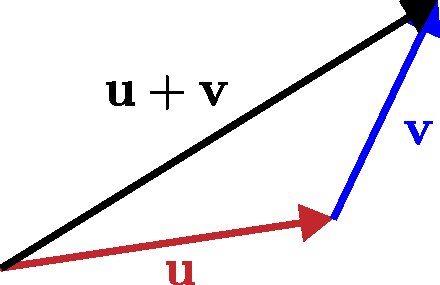
\includegraphics[width=0.35\textwidth]{figs/linear-algebra/triangle-inequality.pdf}
        % \caption{Triangle inequality for norms.}
        % \label{fig:norms}
    \end{figure}
\end{minipage}

\begin{exampleBox}
    \textbf{Example}: For $ \mathbf{v} = \begin{bmatrix}3 \\ -4\end{bmatrix} $:
    \begin{align*}
        \|\mathbf{v}\|_1 &= |3| + |-4| = 7, \\
        \|\mathbf{v}\|_2 &= \sqrt{3^2 + (-4)^2} = 5, \\
        \|\mathbf{v}\|_\infty &= \max\{ |3|, |-4| \} = 4.
    \end{align*}
\end{exampleBox}

\subsection{Norms of Matrices}
Matrix norms extend the concept of vector norms to matrices, providing a measure of the ``size'' or ``magnitude'' of a matrix. Just as vector norms quantify the length of vectors, matrix norms help assess various properties of matrices, such as their behavior under linear transformations, stability in numerical computations, and convergence in iterative methods.

\subsubsection{Induced Matrix Norms}
One fundamental way to define a matrix norm is through an \textbf{induced (operator) norm}, which is derived from a vector norm. Given a vector norm $ \|\cdot\| $ on $ \mathbb{R}^n $ or $ \mathbb{C}^n $, the induced matrix norm for a matrix $ \mathbf{A} \in \mathbb{R}^{m \times n} $ is defined as
\begin{equation*}
    \|\mathbf{A}\| = \max_{\mathbf{x} \neq \mathbf{0}} \frac{\|\mathbf{A}\mathbf{x}\|}{\|\mathbf{x}\|}
\end{equation*}
The induced matrix norm measures the maximum stretching factor of the matrix $ \mathbf{A} $ when it acts as a linear transformation on vectors. Specifically, it identifies the largest possible ratio of the norm of $ \mathbf{A}\mathbf{x} $ to the norm of $ \mathbf{x} $ across all non-zero vectors $ \mathbf{x} $. This tells us how much $ \mathbf{A} $ can amplify a vector.

Induced norms satisfy the following properties:
\begin{itemize}
    \item $\|\mathbf{A}\| \geq 0, \quad \|\mathbf{A}\| = 0 \text{ only if } \mathbf{A} = \mathbf{0}$
    \item $\|c\mathbf{A}\| = |c|\|\mathbf{A}\|$
    \item $\|\mathbf{Ax}\| \leq \|\mathbf{A}\| \|\mathbf{x}\|$ (submultiplicative property)
    \item $\|\mathbf{AB}\| \leq \|\mathbf{A}\| \|\mathbf{B}\|$ (submultiplicative property)
    \item $\|\mathbf{A} + \mathbf{B}\| \leq \|\mathbf{A}\| + \|\mathbf{B}\|$
\end{itemize}
The submultiplicative property is a very important property of induced/operator norms! This property allows us to bound the norm of a product of matrices by the product of their norms and will be very useful in the analysis of iterative methods.

\subsubsection{Common Matrix Norms}
Several matrix norms are commonly used. Below, we take a look at a few of these norms and their interpretations. The first three are induced norms derived from vector norms (and in particular $p$-norms), while the last norm is a matrix-specific norm.
\begin{itemize}
    \item \textbf{1-Norm (Maximum Column Sum)}:
    \begin{equation*}
        \|\mathbf{A}\|_1 = \max_{1 \leq j \leq n} \sum_{i=1}^m |a_{ij}|
    \end{equation*}
    The 1-norm of a matrix is the largest sum of absolute values of the elements in any single column. It represents the maximum effect that $ \mathbf{A} $ can have on the 1-norm of a vector, emphasizing the most  ``influential'' column in terms of contributing to the overall transformation.

    \item \textbf{2-Norm (Spectral Norm)}:
    \begin{equation*}
        \|\mathbf{A}\|_2 = \sigma_{\max}(\mathbf{A})
    \end{equation*}
    where $ \sigma_{\max}(\mathbf{A}) $ denotes the largest singular value of $ \mathbf{A} $. The 2-norm measures the maximum stretching factor of $ \mathbf{A} $ in any direction, corresponding to the largest singular value. It is closely related to the concept of eigenvalues and provides a precise measure of the matrix's action on vectors in terms of scaling.
    
    \item \textbf{Infinity Norm (Maximum Row Sum)}:
    \begin{equation*}
        \|\mathbf{A}\|_\infty = \max_{1 \leq i \leq m} \sum_{j=1}^n |a_{ij}|
    \end{equation*}
    The infinity norm is the largest sum of absolute values of the elements in any single row. It reflects the maximum effect that $ \mathbf{A} $ can have on the infinity norm of a vector, highlighting the most        ``influential'' row in terms of transformation impact.
    
    \item \textbf{Frobenius Norm}:
    \begin{equation*}
        \|\mathbf{A}\|_F = \sqrt{\sum_{i=1}^m \sum_{j=1}^n a_{ij}^2}
    \end{equation*}
    Again, this is NOT an induced norm. The Frobenius norm is very similar to the Euclidean norm (which is defined for vectors). It measures the ``overall size'' of the matrix by taking the square root of the sum of the squares of all its entries. This norm is particularly useful in applications where the collective magnitude of all matrix elements is of interest, such as in least squares problems and matrix approximations.
\end{itemize}

\subsubsection{Relationships Between Matrix Norms}
For any matrix $ \mathbf{A} $ of size $ m \times n $ and rank $ r $, the following inequalities hold:
\begin{align*}
    \|\mathbf{A}\|_2 &\leq \|\mathbf{A}\|_F \leq \sqrt{r}\,\|\mathbf{A}\|_2, \\
    \|\mathbf{A}\|_2 &\leq \sqrt{\|\mathbf{A}\|_1 \, \|\mathbf{A}\|_\infty}.
\end{align*}

\section{Introduction to Systems of Linear Equations}
Linear systems arise in many scientific and engineering applications (even in seemingly nonlinear cases, we can Taylor expand to a locally linear system), so we should develop tools to numerically solve them. The general form of a linear system is
\begin{equation}
    \mathbf{A}\mathbf{x} = \mathbf{b}
    \label{eq:linear-system}
\end{equation}
where $ \mathbf{A} \in \mathbb{R}^{M \times N} $ is a known coefficient matrix, $ \mathbf{x} \in \mathbb{R}^N $ is the vector of unknowns, and $ \mathbf{b} \in \mathbb{R}^M $ is a known vector. The goal is to find $ \mathbf{x} $ that satisfies this equation. We know from linear algebra that this linear system has a unique solution for a given $\mathbf{b}$ if and only if $ \mathbf{A} $ is square ($M=N$) and has full rank (i.e., $\operatorname{rank}(\mathbf{A})=N$). Otherwise, the system may have no solution or infinitely many solutions. If $M\ne N$, we typically seek a least-squares ($M>N$) or minimum-norm ($M<N$) solution.


\subsection{Condition Number}
Before looking at specific direct and iterative methods, we introduce the notion of the \textbf{condition number} of a matrix $\mathbf{A}$, denoted $\kappa(\mathbf{A})$, which helps us understand the sensitivity of a linear system to perturbations and numerical errors. We hope that for our linear system $\mathbf{A}\mathbf{x} = \mathbf{b}$, small perturbations in $\mathbf{b}$ will lead to small changes in $\mathbf{x}$. Such a system is said to be well-conditioned. However, if small perturbations in $\mathbf{b}$ lead to large changes in $\mathbf{x}$, the system is said to be ill-conditioned. The meaning of ``small'' and ``large'' changes depending on the context (e.g., it could be relative or absolute). The condition number quantifies this sensitivity.

To define the condition number, we consider a linear system $ \mathbf{A}\mathbf{x} = \mathbf{b} $ with an exact solution $ \mathbf{x} = \mathbf{A}^{-1}\mathbf{b} $. If we add a small perturbation (error) $\delta\mathbf{b}$ to $\mathbf{b}$, then the solution vector $\mathbf{x}$ will also change by some amount $\delta\mathbf{x}$ (which we think of as the error in $\mathbf{x}$ since the original perturbation is assumed to represent an error) so that the linear system remains satisfied:
\begin{equation*}
    \mathbf{A}\left(\mathbf{x} + \delta\mathbf{x}\right) = \mathbf{b} + \delta\mathbf{b}
    \implies 
    \delta\mathbf{x} = \mathbf{A}^{-1}\delta\mathbf{b}
\end{equation*}
Taking the $p$-norm of both sides, we have
\begin{equation*}
    \|\delta\mathbf{x}\|_p = \|\mathbf{A}^{-1}\delta\mathbf{b}\|_p \leq \|\mathbf{A}^{-1}\|_p \|\delta\mathbf{b}\|_p
\end{equation*}
where the inequality follows from the submultiplicative property of matrix norms. We also have $\|\mathbf{b}\|_p = \|\mathbf{A}\mathbf{x}\|_p \le \|\mathbf{A}\|_p \, \|\mathbf{x}\|_p$, hence $\|\mathbf{x}\|_p \ge \|\mathbf{b}\|_p/\|\mathbf{A}\|_p$. Dividing the two inequalities, we arrive at an expression for the relative error in the solution:
\begin{equation*}
    \frac{\|\delta\mathbf{x}\|_p}{\|\mathbf{x}\|_p} \leq \|\mathbf{A}\|_p \|\mathbf{A}^{-1}\|_p \frac{\|\delta\mathbf{b}\|_p}{\|\mathbf{b}\|_p}
\end{equation*}
This motivates the definition of the condition number of $\mathbf{A}$ as
\begin{equation*}
    \kappa_p(\mathbf{A}) = \|\mathbf{A}\|_p \|\mathbf{A}^{-1}\|_p
\end{equation*}
where we add a subscript $p$ on $\kappa$ to denote the norm used and to emphasize that its value depends on the choice of norm (but the qualitative behavior is the same across norms). If $\mathbf{A}$ is singular, $\kappa_p(\mathbf{A}) = \infty$. We note that clearly $\kappa_p(\mathbf{A}) \geq 1$ since $\|\mathbf{A}\|_p \|\mathbf{A}^{-1}\|_p \geq \|\mathbf{A} \mathbf{A}^{-1}\|_p = \|\mathbf{I}\|_p = 1$. Moreover, a matrix with a large condition number (an ``ill-conditioned'' matrix) indicates that the linear system is more sensitive to perturbations and numerical errors, while a matrix with a small condition number (a ``well-conditioned'' matrix) indicates greater numerical robustness. As a practical rule of thumb for backward-stable solvers (e.g., Gaussian elimination with partial pivoting), the number of correct digits $\approx$ (working-precision digits) $-\log_{10}\kappa(\mathbf{A})$, and the relative forward error is typically $O(\kappa(\mathbf{A})\,\varepsilon_{\mathrm{mach}})$. A small residual $\|\mathbf{r}\| = \|\mathbf{b}-\mathbf{A}\hat{\mathbf{x}}\|$ does not guarantee a small error when $\kappa(\mathbf{A})$ is large; roughly,
\[ \frac{\|\hat{\mathbf{x}}-\mathbf{x}\|}{\|\mathbf{x}\|} \lesssim \kappa(\mathbf{A})\,\frac{\|\mathbf{r}\|}{\|\mathbf{b}\|}. \]

Let's take a look at the condition number for the 2-norm specifically. Here, the condition number is
\begin{equation*}
    \kappa_2(\mathbf{A}) = \|\mathbf{A}\|_2 \|\mathbf{A}^{-1}\|_2 = \frac{\sigma_{\text{max}}(\mathbf{A})}{\sigma_{\text{min}}(\mathbf{A})}
\end{equation*}
where $\sigma_{\text{max}}(\mathbf{A})$ and $\sigma_{\text{min}}(\mathbf{A})$ are the largest and smallest singular values of $\mathbf{A}$, respectively. For $\mathbf{A} \succ 0$,\footnote{If $\mathbf{A}$ is normal ($\mathbf{A}\mathbf{A}^* = \mathbf{A}^*\mathbf{A}$) over $\mathbb{C}$, then $\sigma_i(\mathbf{A}) = |\lambda_i(\mathbf{A})|$ and $\kappa_2(\mathbf{A}) = \max_i |\lambda_i(\mathbf{A})|/\min_i |\lambda_i(\mathbf{A})|$.} this is equivalent to
\begin{equation*}
    \kappa_2(\mathbf{A}) = \frac{\lambda_{\text{max}}(\mathbf{A})}{\lambda_{\text{min}}(\mathbf{A})}
\end{equation*}
where $\lambda_{\text{max}}(\mathbf{A})$ and $\lambda_{\text{min}}(\mathbf{A})$ are the largest and smallest eigenvalues of $\mathbf{A}$, respectively.

\textbf{Preconditioning}\quad When solving linear systems numerically, we often encounter ill-conditioned matrices. One way to mitigate the effects of ill-conditioning is through \textbf{preconditioning}. Preconditioning transforms $ \mathbf{A}\mathbf{x} = \mathbf{b} $ into a system with more favorable spectral properties. Common forms are left $(\mathbf{P}^{-1}\mathbf{A})\mathbf{x} = \mathbf{P}^{-1}\mathbf{b}$, right $\ \mathbf{A}(\mathbf{P}^{-1}\mathbf{y}) = \mathbf{b}$ with $\mathbf{x}=\mathbf{P}^{-1}\mathbf{y}$, and symmetric $\ \mathbf{P}^{-1/2}\mathbf{A}\mathbf{P}^{-1/2}\mathbf{z} = \mathbf{P}^{-1/2}\mathbf{b}$ with $\mathbf{x}=\mathbf{P}^{-1/2}\mathbf{z}$. Examples include Jacobi (diagonal), incomplete LU/Cholesky (ILU/IC), and algebraic multigrid (AMG). The goal is to cluster eigenvalues and reduce the effective condition number to accelerate and stabilize iterative methods.

Even simpler than preconditioning is \textbf{scaling} (often called equilibration), which rescales rows and/or columns to reduce element-wise dynamic range and improve pivoting. A common heuristic is to equalize row/column $\infty$-norms. This helps numerics and pivoting but does not magically fix ill-conditioning rooted in the model; think nondimensionalization and consistent units (ChemE context: Pa vs bar, mol vs kmol).

\begin{exampleBox}
    \textbf{Example:} Consider the matrix
    \begin{equation*}
        \mathbf{A} = \begin{bmatrix}
        10^{14} & 0 \\
        0 & 10^{-9}
        \end{bmatrix}
    \end{equation*}
    The condition number of this matrix with respect to the 2-norm is
    \begin{equation*}
        \kappa_2(\mathbf{A}) = \frac{\lambda_{\text{max}}(\mathbf{A})}{\lambda_{\text{min}}(\mathbf{A})} = \frac{10^{14}}{10^{-9}} = 10^{23}
    \end{equation*}
    which means that $\mathbf{A}$ is severely ill-conditioned. Such a high condition number implies that even tiny perturbations in $\mathbf{b}$ can lead to enormous errors in the computed solution $\mathbf{x}$.

    To mitigate this issue, we can apply scaling by rescaling the rows of $\mathbf{A}$ to reduce the condition number. Specifically, we divide each row by the maximum absolute value in that row. For matrix $\mathbf{A}$, the scaling factors for the rows are $10^{14}$ and $10^{-9}$, respectively. We define a diagonal scaling matrix $\mathbf{D}$ as
    \begin{equation*}
    \mathbf{D} = \begin{bmatrix}
    10^{-14} & 0 \\
    0 & 10^{9}
    \end{bmatrix}
    \end{equation*}
    Applying the scaling, we obtain the scaled matrix $\mathbf{A}_{\text{scaled}}$:
    \begin{equation*}
    \mathbf{A}_{\text{scaled}} = \mathbf{D} \mathbf{A} = \begin{bmatrix}
    10^{-14} & 0 \\
    0 & 10^{9}
    \end{bmatrix} \begin{bmatrix}
    10^{14} & 0 \\
    0 & 10^{-9}
    \end{bmatrix} = \begin{bmatrix}
    1 & 0 \\
    0 & 1
    \end{bmatrix}
    \end{equation*}
    The left-scaling forms the equivalent system $\mathbf{D}\mathbf{A}\mathbf{x} = \mathbf{D}\mathbf{b}$ (same solution $\mathbf{x}$). Here, because $\mathbf{A}$ is diagonal, $\mathbf{D}\mathbf{A} = \mathbf{I}$. In general, equilibration reduces dynamic range and can reduce $\kappa$, but need not drive it to 1.

    The condition number of the scaled matrix is now
    \begin{equation*}
        \kappa_2(\mathbf{A}_{\text{scaled}}) = \frac{\lambda_{\text{max}}(\mathbf{A}_{\text{scaled}})}{\lambda_{\text{min}}(\mathbf{A}_{\text{scaled}})} = \frac{1}{1} = 1
    \end{equation*}
    which means that $\mathbf{A}_{\text{scaled}}$ is perfectly conditioned. This dramatic reduction shows how scaling can improve numerical behavior in favorable cases (in this case, $\mathbf{A}$ is diagonal, so $\mathbf{D} = \mathbf{A}^{-1}$ is an exact preconditioner, hence the perfect condition number). In general, scaling is often helpful for stability and pivoting, but it does not eliminate all ill-conditioning.
\end{exampleBox}

\begin{warningBox}
    \textbf{Warning:} Preconditioning/scaling improves the matrix the algorithm sees (e.g., reduces $\kappa(P^{-1}A)$), which speeds and stabilizes iterations, but it \emph{doesn't change the intrinsic sensitivity} of the original mapping $\mathbf{x}=\mathbf{A}^{-1}\mathbf{b}$ to perturbations in $b$. So it helps the solver's numerics, not the problem's conditioning.
\end{warningBox}



\section{Invertibility and Determinants}
\subsection{Determinant}
For a square matrix $ \mathbf{A} \in \mathbb{R}^{n\times n} $, the \textbf{determinant} $ \det(\mathbf{A}) $ is a scalar value that can tell us a lot about the matrix's properties. Geometrically, it represents the signed volume-scaling factor of the linear transformation described by $ \mathbf{A} $. If $ |\det(\mathbf{A})| = 2 $, the transformation doubles the volume of a region, while if $ |\det(\mathbf{A})| = 0.5 $, it halves the volume. The sign of the determinant tells us whether the transformation preserves or reverses orientation. A positive determinant means the orientation is preserved, while a negative determinant means it's flipped (think of it as turning a shape ``inside-out'' like a reflection). If $ \det(\mathbf{A}) = 0 $, the transformation collapses the space into a lower dimension (e.g., squashing a 2D square into a line segment). When this happens, information is lost, and you can't reverse the transformation.
This offers insight into the fact that a matrix is \textbf{invertible if and only if its determinant is non-zero}.


The determinant has several important properties, including $ \det(\mathbf{A}^\top) = \det(\mathbf{A}) $, the multiplicative property $ \det(\mathbf{AB}) = \det(\mathbf{A})\det(\mathbf{B}) $, and the fact that for an invertible matrix, $ \det(\mathbf{A}^{-1}) = 1 / \det(\mathbf{A}) $.

For a $2\times 2$ matrix, the formula is
\begin{equation*}
    \det\!\left(\begin{bmatrix} a & b \\ c & d \end{bmatrix}\right) = ad - bc
\end{equation*}
For a $3\times 3$ matrix, one common method is cofactor expansion along the first row:
\begin{align*}
    \det\!\left(\begin{bmatrix} a & b & c \\ d & e & f \\ g & h & i \end{bmatrix}\right) &= a \det\!\left(\begin{bmatrix} e & f \\ h & i \end{bmatrix}\right) - b \det\!\left(\begin{bmatrix} d & f \\ g & i \end{bmatrix}\right) + c \det\!\left(\begin{bmatrix} d & e \\ g & h \end{bmatrix}\right) \\ &= a(ei - fh) - b(di - fg) + c(dh - eg)
\end{align*}
The determinant of a general $n \times n$ matrix can be defined recursively via Laplace expansion, which expresses it as a signed sum of the entries of any chosen row or column times the determinants of their $(n-1) \times (n-1)$ minors. This recursion reduces ultimately to the $2 \times 2$ case. However, in practice, Laplace expansion is only used for small matrices; large determinants are almost always computed using Gaussian elimination or LU decomposition instead.


\subsection{Inverse of a Matrix}
Conceptually, the inverse of a matrix, denoted $ \mathbf{A}^{-1} $, is an operator that reverses the linear transformation performed by the original matrix $ \mathbf{A} $. If $ \mathbf{A} $ transforms a vector $ \mathbf{x} $ into $ \mathbf{y} $ (i.e., $ \mathbf{y} = \mathbf{A}\mathbf{x} $), then its inverse $ \mathbf{A}^{-1} $ transforms $ \mathbf{y} $ back to the original vector $ \mathbf{x} $ (i.e., $ \mathbf{x} = \mathbf{A}^{-1}\mathbf{y} $).

Formally, a square matrix $ \mathbf{A} $ is \textbf{invertible} (or \textbf{non-singular}) if there exists a matrix $ \mathbf{A}^{-1} $ such that:
\begin{equation*}
    \mathbf{A}\mathbf{A}^{-1} = \mathbf{A}^{-1}\mathbf{A} = \mathbf{I}
\end{equation*}
where $ \mathbf{I} $ is the identity matrix. This property is analogous to a number and its reciprocal (e.g., $ 5 \cdot 5^{-1} = 1 $).

A matrix is invertible if and only if its determinant is non-zero ($ \det(\mathbf{A}) \neq 0 $). If the determinant is zero, the matrix is singular, meaning its transformation is irreversible because it collapses the space into a lower dimension (e.g., mapping a 2D plane onto a line), and the original vector cannot be uniquely recovered.

This ``undoing'' capability is fundamental for solving systems of linear equations. A system represented as $ \mathbf{A}\mathbf{x} = \mathbf{b} $ can be solved for the unknown vector $ \mathbf{x} $ by applying the inverse: $ \mathbf{A}^{-1}\mathbf{A}\mathbf{x} = \mathbf{A}^{-1}\mathbf{b} $, which simplifies to $ \mathbf{x} = \mathbf{A}^{-1}\mathbf{b} $.

Important properties of inverses include $(\mathbf{A}\mathbf{B})^{-1} = \mathbf{B}^{-1}\mathbf{A}^{-1}$ (note the reversed order) and $(\mathbf{A}^\top)^{-1} = (\mathbf{A}^{-1})^\top$. For a $2\times 2$ matrix, the inverse can be calculated directly:
\begin{equation*}
    \text{If } \mathbf{A} = \begin{bmatrix} a & b \\ c & d \end{bmatrix}, \text{ then } \mathbf{A}^{-1} = \frac{1}{ad-bc} \begin{bmatrix} d & -b \\ -c & a \end{bmatrix}, \quad \text{provided } ad-bc \neq 0
\end{equation*}
While the $2 \times 2$ formula is simple, computing the inverse for a general $n \times n$ matrix is a numerically intensive task. In practice, one typically avoids computing the inverse explicitly. For problems like solving $\mathbf{A}\mathbf{x} = \mathbf{b}$, it is both more efficient and more numerically stable to solve the system directly using matrix factorization or other methods instead, which we will discuss in more detail later.




\section{Existence and Uniqueness of Solutions}

\subsection{Linear Combinations and Span} % SS: probably we should explain this later, after introducing the vector space.
A \textbf{linear combination} of vectors $ \mathbf{v}_1, \mathbf{v}_2, \ldots, \mathbf{v}_k $ is an expression of the form:
\begin{equation*}
    \mathbf{w} = c_1 \mathbf{v}_1 + c_2 \mathbf{v}_2 + \ldots + c_k \mathbf{v}_k
\end{equation*}
where $ c_1, c_2, \ldots, c_k $ are scalars. The set of all possible linear combinations of $ \mathbf{v}_1, \ldots, \mathbf{v}_k $ is called their \textbf{span}:
\begin{equation*}
    \text{span}\{\mathbf{v}_1, \ldots, \mathbf{v}_k\} = \left\{ \sum_{i=1}^k c_i \mathbf{v}_i \mid c_i \in \mathbb{R} \text{ or } \mathbb{C} \right\}
\end{equation*}

\begin{exampleBox}
    \textbf{Example}: Consider vectors $ \mathbf{v}_1 = \begin{bmatrix}1 \\ 0\end{bmatrix} $ and $ \mathbf{v}_2 = \begin{bmatrix}0 \\ 1\end{bmatrix} $ in $ \mathbb{R}^2 $. Their span is the entire $ \mathbb{R}^2 $ plane since any vector $ \mathbf{w} = \begin{bmatrix}w_1 \\ w_2\end{bmatrix} $ can be written as $ w_1 \mathbf{v}_1 + w_2 \mathbf{v}_2 $
\end{exampleBox}

\subsection{Linear Independence and Basis}
Vectors $ \mathbf{v}_1, \ldots, \mathbf{v}_k $ are \textbf{linearly independent} if the only solution to
\begin{equation*}
    c_1 \mathbf{v}_1 + c_2 \mathbf{v}_2 + \ldots + c_k \mathbf{v}_k = \mathbf{0}
\end{equation*}
is $ c_1 = c_2 = \ldots = c_k = 0 $.

A set of vectors that is linearly independent and spans the vector space is called a \textbf{basis}. The number of vectors in a basis equals the \textbf{dimension} of the space.

% \subsection{The Zero Vector}
% The \textbf{zero vector} $ \mathbf{0} $ in $ \mathbb{R}^n $ is:
% \begin{equation*}
%     \mathbf{0} = \begin{bmatrix}0 \\ 0 \\ \vdots \\ 0\end{bmatrix}
% \end{equation*}
% It acts as the additive identity: $ \mathbf{v} + \mathbf{0} = \mathbf{v} $.

\subsection{The Unit Vectors}
The \textbf{unit vectors} in $ \mathbb{R}^n $ are:
\begin{equation*}
    \mathbf{e}_i = \begin{bmatrix}0 \\ \vdots \\ 1 \\ \vdots \\ 0\end{bmatrix}, \quad \text{where } (\mathbf{e}_{i})_j = \begin{cases} 1 & \text{if } i = j \\ 0 & \text{otherwise} \end{cases}
\end{equation*}
The unit vectors form a basis for $ \mathbb{R}^n $, meaning any vector $ \mathbf{v} $ can be written as a linear combination of the unit vectors.
\begin{exampleBox}
    \textbf{Example}: In $ \mathbb{R}^3 $, the unit vectors are $ \mathbf{e}_1 = \begin{bmatrix}1 \\ 0 \\ 0\end{bmatrix} $, $ \mathbf{e}_2 = \begin{bmatrix}0 \\ 1 \\ 0\end{bmatrix} $, and $ \mathbf{e}_3 = \begin{bmatrix}0 \\ 0 \\ 1\end{bmatrix} $.
\end{exampleBox}

\subsection{Properties of Vector Spaces}\label{sec:vector-space}
For all $ \mathbf{u}, \mathbf{v}, \mathbf{w} \in \mathbb{R}^n $ and scalars $ c, d \in \mathbb{R} $, the following hold:
\begin{enumerate}
    \item $ \mathbf{u} + \mathbf{v} = \mathbf{v} + \mathbf{u} $ (commutativity)
    \item $ (\mathbf{u} + \mathbf{v}) + \mathbf{w} = \mathbf{u} + (\mathbf{v} + \mathbf{w}) $ (associativity)
    \item $ \mathbf{v} + \mathbf{0} = \mathbf{v} $ (additive identity)
    \item $ \mathbf{v} + (-\mathbf{v}) = \mathbf{0} $ (additive inverse)
    \item $ c(d\mathbf{v}) = (cd)\mathbf{v} $ (associativity of scalar multiplication)
    \item $ (c + d)\mathbf{v} = c\mathbf{v} + d\mathbf{v} $ (distributivity over scalars)
    \item $ c(\mathbf{v} + \mathbf{w}) = c\mathbf{v} + c\mathbf{w} $ (distributivity over vectors)
    \item $ 1\mathbf{v} = \mathbf{v} $ (multiplicative identity)
\end{enumerate}

\subsection{Orthogonality}
Vectors $ \mathbf{u}, \mathbf{v} \in \mathbb{R}^n $ are \textbf{orthogonal} if $ \mathbf{u}^\top \mathbf{v} = 0 $. A set of vectors is \textbf{orthonormal} if vectors are mutually orthogonal and each has unit norm. A square matrix $ \mathbf{Q} $ is \textbf{orthogonal} if $ \mathbf{Q}^\top \mathbf{Q} = \mathbf{Q}\mathbf{Q}^\top = \mathbf{I} $, which implies $ \mathbf{Q}^{-1} = \mathbf{Q}^\top $ and that $ \|\mathbf{Q}\mathbf{x}\|_2 = \|\mathbf{x}\|_2 $ for all $ \mathbf{x} $.



\subsection{The four fundamental subspaces}
We next formalize when a linear system has a solution and when that solution is unique. When needed, we denote by $\mathbf{A}_i^c$ the $i$-th column and by $\mathbf{A}_i^r$ the $i$-th row.
For a matrix $\mathbf{A}\in\mathbb{R}^{N\times M}$ there are four canonical subspaces:
\begin{enumerate}
    \item \textbf{Column space (range):} $\displaystyle \mathcal{R}(\mathbf{A})=\operatorname{span}\{\mathbf{A}_1^c,\dots,\mathbf{A}_M^c\}\subseteq\mathbb{R}^N$
    \item \textbf{Null space (kernel):} $\displaystyle \mathcal{N}(\mathbf{A})=\{\mathbf{x}\in\mathbb{R}^M:\ \mathbf{A}\mathbf{x}=\mathbf{0}\}$;
    \item \textbf{Row space:} $\displaystyle \mathcal{R}(\mathbf{A}^{\top})=\operatorname{span}\{\mathbf{A}_1^r,\dots,\mathbf{A}_N^r\}\subseteq\mathbb{R}^M$
    \item \textbf{Left null space:} $\displaystyle \mathcal{N}(\mathbf{A}^{\top})=\{\mathbf{y}\in\mathbb{R}^N:\ \mathbf{A}^{\top}\mathbf{y}=\mathbf{0}\}$
\end{enumerate}
These subspaces organize the two core questions for a system $\mathbf{A}\mathbf{x}=\mathbf{b}$: \emph{existence} (is $\mathbf{b}$ achievable?) and \emph{uniqueness} (if achievable, is the achiever $\mathbf{x}$ unique?). 

Think of $\mathbf{A}:\mathbb{R}^M\to\mathbb{R}^N$ as a machine that takes an input vector $\mathbf{x}$ and produces an output $\mathbf{b}=\mathbf{A}\mathbf{x}$. The set of all outputs the machine can possibly produce is the \emph{column space} $\mathcal{R}(\mathbf{A})$. Directions in input space that the machine completely ignores (they map to $\mathbf{0}$) form the \emph{null space} $\mathcal{N}(\mathbf{A})$. Thus:
\[
\text{existence is about }\mathbf{b}\in\mathcal{R}(\mathbf{A}),\qquad
\text{uniqueness is about }\mathcal{N}(\mathbf{A})=\{\mathbf{0}\}
\]
The four subspaces come in orthogonal pairs:
\[
\mathcal{R}(\mathbf{A})=\mathcal{N}(\mathbf{A}^{\top})^{\perp}
\quad\text{and}\quad
\mathcal{R}(\mathbf{A}^{\top})=\mathcal{N}(\mathbf{A})^{\perp}
\]
Consequently,
\[
\mathbb{R}^N=\mathcal{R}(\mathbf{A})\oplus \mathcal{N}(\mathbf{A}^{\top}),
\qquad
\mathbb{R}^M=\mathcal{R}(\mathbf{A}^{\top})\oplus \mathcal{N}(\mathbf{A})
\]
In words, this means that for an $N\times M$ matrix $\mathbf{A}$, every vector in $\mathbb{R}^N$ can be written uniquely as a sum of something in the column space $\mathcal R(\mathbf{A})$ and something in the left null space $\mathcal N(\mathbf{A}^\top)$. Likewise, every vector in $\mathbb{R}^M$ splits uniquely into a part in the row space $\mathcal R(\mathbf{A}^\top)$ and a part in the null space $\mathcal N(\mathbf{A})$. As a dimension check this yields
\[
\dim\mathcal{R}(\mathbf{A})+\dim\mathcal{N}(\mathbf{A}^{\top})=N
\qquad
\dim\mathcal{R}(\mathbf{A}^{\top})+\dim\mathcal{N}(\mathbf{A})=M
\]
It is also a basic fact that row rank equals column rank:
\[
\operatorname{rank}(\mathbf{A})=\dim\mathcal{R}(\mathbf{A})
=\dim\mathcal{R}(\mathbf{A}^{\top})
=\operatorname{rank}(\mathbf{A}^{\top})
\]

\begin{theoremBox}
\textbf{Theorem (existence via the column space):} A solution to $\mathbf{A}\mathbf{x}=\mathbf{b}$ exists for a given $\mathbf{b}$ if and only if $\mathbf{b}\in\mathcal{R}(\mathbf{A})$.

\textit{Proof.}\; Using the column view,
\[
\mathbf{A}\mathbf{x}=\sum_{i=1}^{M}x_i\,\mathbf{A}_i^c
\]
If $\mathbf{b}\in\mathcal{R}(\mathbf{A})$, then by definition there exist coefficients $x_i$ so that the sum equals $\mathbf{b}$, hence a solution exists. Conversely, if $\mathbf{A}\mathbf{x}=\mathbf{b}$ for some $\mathbf{x}$, then $\mathbf{b}$ is a linear combination of the columns of $\mathbf{A}$, so $\mathbf{b}\in\mathcal{R}(\mathbf{A})$.

\end{theoremBox}

We can also look at things geometrically. The column space is a subspace (a line/plane/higher-dimensional flat) inside $\mathbb{R}^N$. Asking for a solution is asking whether $\mathbf{b}$ lies \emph{on} that flat. If not, there is no exact solution; if yes, there is at least one.

\begin{exampleBox}
\textbf{Example (existence).} Let
\[
\mathbf{A}=\begin{bmatrix}1&0&0\\ 0&0&0\\ 0&0&0\end{bmatrix},\quad
\mathbf{b}_1=\begin{bmatrix}1\\0\\0\end{bmatrix},\quad
\mathbf{b}_2=\begin{bmatrix}0\\1\\0\end{bmatrix}.
\]
The column space is $\mathcal{R}(\mathbf{A})=\operatorname{span}\{(1,0,0)^{\top}\}$, a $1$-dimensional line in $\mathbb{R}^3$. Thus $\mathbf{b}_1$ lies on that line, so solutions exist (e.g., $x_1=1$ and $x_2,x_3$ arbitrary). The vector $\mathbf{b}_2$ lies off the line, so no solution exists.
\end{exampleBox}

\subsection{Consistency via the left null space (Fredholm alternative)}
The system $\mathbf{A}\mathbf{x}=\mathbf{b}$ is solvable if and only if $\mathbf{b}\perp \mathcal{N}(\mathbf{A}^{\top})$; equivalently, $\mathbf{b}\in\mathcal{R}(\mathbf{A})$. In practice this gives a test: if $\{\mathbf{y}_1,\dots,\mathbf{y}_k\}$ is a basis of $\mathcal{N}(\mathbf{A}^{\top})$, then $\mathbf{A}\mathbf{x}=\mathbf{b}$ is consistent precisely when $\mathbf{y}_j^{\top}\mathbf{b}=0$ for all $j$.

\begin{theoremBox}
\textbf{Theorem (Uniqueness via the null space):} If a solution to $\mathbf{A}\mathbf{x}=\mathbf{b}$ exists, it is unique if and only if $\dim\mathcal{N}(\mathbf{A})=0$ (equivalently, $\mathcal{N}(\mathbf{A})=\{\mathbf{0}\}$).

\textit{Proof ($\Leftarrow$).}\; If $\mathcal{N}(\mathbf{A})=\{\mathbf{0}\}$ and $\mathbf{A}\mathbf{x}=\mathbf{A}\mathbf{y}=\mathbf{b}$, then $\mathbf{A}(\mathbf{x}-\mathbf{y})=\mathbf{0}$, hence $\mathbf{x}-\mathbf{y}=\mathbf{0}$ and $\mathbf{x}=\mathbf{y}$.

\textit{Proof ($\Rightarrow$).}\; Suppose a solution exists and is unique. If there were a nonzero $\mathbf{x}^{H}\in\mathcal{N}(\mathbf{A})$, then for any particular solution $\mathbf{x}^{P}$, the vector $\mathbf{x}^{P}+\mathbf{x}^{H}$ would be a distinct solution, a contradiction.
\end{theoremBox}

\begin{exampleBox}
\textbf{Example (uniqueness with $M<N$):} Consider
\[
\mathbf{A}=\begin{bmatrix}
1&0\\ 1&0\\ 1&0\\ 0&1
\end{bmatrix}\in\mathbb{R}^{4\times 2}.
\]
The columns are $\mathbf{c}_1=(1,1,1,0)^{\top}$ and $\mathbf{c}_2=(0,0,0,1)^{\top}$, which are linearly independent. Hence $\mathcal{N}(\mathbf{A})=\{\mathbf{0}\}$ and any consistent system has a unique solution. Concretely, a right-hand side $\mathbf{b}=(b_1,b_2,b_3,b_4)^{\top}$ is in $\mathcal{R}(\mathbf{A})$ iff $b_1=b_2=b_3$; when this holds, the unique solution is $x_1=b_1$ and $x_2=b_4$.
\end{exampleBox}

\subsection{Rank and nullity} The rank and nullity of $\mathbf{A}\in\mathbb{R}^{N\times M}$ are
\[
\operatorname{rank}(\mathbf{A})=\dim\mathcal{R}(\mathbf{A}),
\qquad
\operatorname{nullity}(\mathbf{A})=\dim\mathcal{N}(\mathbf{A}).
\]
Always, $\operatorname{rank}(\mathbf{A})\le \min\{M,N\}$. We say that $\mathbf{A}$ has full column rank if $\operatorname{rank}(\mathbf{A})=M$ and full row rank if $\operatorname{rank}(\mathbf{A})=N$.

\begin{theoremBox}
\textbf{Rank--nullity theorem:}
For every $\mathbf{A}\in\mathbb{R}^{N\times M}$,
\[
\operatorname{rank}(\mathbf{A})+\operatorname{nullity}(\mathbf{A})=M
\]
\end{theoremBox}
An immediate consequence of the rank-nullity theorem is that if $M>N$ (more variables than equations), then $\operatorname{rank}(\mathbf{A})\le N$ so $\operatorname{nullity}(\mathbf{A})\ge M-N>0$. Thus, whenever a solution exists, it cannot be unique. Conversely, if $N>M$ (more equations than variables), uniqueness (when consistent) is possible exactly when $\mathbf{A}$ has full column rank $M$, but solvability for \emph{every} $\mathbf{b}\in\mathbb{R}^N$ is impossible since that would require rank $N>M$.

\subsection{Square case and invertibility} When $\mathbf{A}\in\mathbb{R}^{N\times N}$, the following are equivalent for a square system:
\begin{itemize}
    \item for every $\mathbf{b}\in\mathbb{R}^N$ there exists a \emph{unique} solution of $\mathbf{A}\mathbf{x}=\mathbf{b}$
    \item $\mathbf{A}$ is invertible
    \item $\det(\mathbf{A})\neq 0$
    \item $\operatorname{rank}(\mathbf{A})=N$
    \item $\dim\mathcal{N}(\mathbf{A})=0$
\end{itemize}
Each statement enforces both existence (full row rank) and uniqueness (full column rank), which coincide in the square case.

Now, we return to the problem of finding the solution of \autoref{eq:linear-system}. At first glance, it might seem straightforward to solve for $ \mathbf{x} $ by simply computing the inverse of $ \mathbf{A} $, since theoretically, if $ \mathbf{A} $ is invertible, the solution is given by
\begin{equation*}
    \mathbf{x} = \mathbf{A}^{-1}\mathbf{b}
\end{equation*}
However, in practice, computing $ \mathbf{A}^{-1} $ directly is generally avoided for several important reasons: (1) computational cost, (2) numerical stability, and (3) memory requirements. For these reasons, numerical methods focus on solving linear systems without explicitly computing the inverse of $ \mathbf{A} $. There are two primary classes of numerical methods for solving linear systems: \textbf{direct methods} and \textbf{iterative methods}. Each has its own advantages and is suitable for different types of problems.


\section{Numerical Solution of Linear Systems: Direct Methods}
\label{sec:num_sol_linear_direct}
Direct methods are named for their ability to (given no round-off errors) determine the exact solution to a linear system within a finite number of steps. In practical applications, however, finite precision limits these methods to producing only approximate solutions.

Direct methods take advantage of the fact that we can easily solve the system \autoref{eq:linear-system} when $ \mathbf{A} $ is upper triangular by using back substitution. Direct methods typically involve some variant of Gaussian elimination, which is a systematic procedure for transforming the coefficient matrix $ \mathbf{A} $ into an upper triangular form in order to be able to solve the system by back substitution. 

\subsection{Back Substitution}
Back substitution is a method for solving linear systems of equations that are in upper triangular form. The idea is to start with the last equation and solve for the last unknown, then use that result to solve for the second-to-last unknown, and so on (working backwards, hence the name). In mathematical terms, this is expressed as
\begin{equation*}
    x_i = \frac{1}{a_{ii}} \left( b_i - \sum_{j=i+1}^{n} a_{ij} x_j \right) \quad \text{for } i = n, n-1, \dots, 1
\end{equation*}
where $ a_{ij} $ are the elements of the upper triangular matrix $ \mathbf{A} \in \mathbb{R}^{n \times n} $, $ b_i $ are the elements of the vector $ \mathbf{b} $, and $ x_i $ are the unknowns we are solving for. Notice that the formula for $ x_k $ for some $k < n$ relies on the values of $ x_{k+1}, x_{k+2}, \dots, x_n $, which is why we must work backwards.

\begin{exampleBox}
    \textbf{Example}: Consider the following linear system:
    \begin{equation*}
        \begin{bmatrix}
        1 & 2 & 3 \\
        0 & 4 & 5 \\
        0 & 0 & 6
        \end{bmatrix}
        \begin{bmatrix}
        x_1 \\ x_2 \\ x_3
        \end{bmatrix}
        =
        \begin{bmatrix}
        1 \\ 13 \\ 6
        \end{bmatrix}
    \end{equation*}
    Let's work backwards naively to gain some intuition. The last equation is $ 6x_3 = 6 $, so $ x_3 = 6/6 = 1 $. The second-to-last equation is $ 4x_2 + 5(1) = 13 $, so $ x_2 = (13 - 5)/4 = 2 $. Finally, the first equation is $ x_1 + 2(2) + 3(1) = 1 $, so $ x_1 = 1 - 4 - 3 = -6 $. Therefore, the solution to the system is $ x_1 = -6 $, $ x_2 = 2 $, and $ x_3 = 1 $.

    We can also just directly apply the formula for back substitution (note that the formula is the exact same as the naive/intuitive approach given above, just written in a way that generalizes to larger systems):
    \begin{align*}
        x_3 & = \frac{1}{6} \left( 6 - 0 \right) = 1 \\
        x_2 & = \frac{1}{4} \left( 13 - 5(1) \right) = 2 \\
        x_1 & = \frac{1}{1} \left( 1 - 2(2) - 3(1) \right) = -6
    \end{align*}
\end{exampleBox}

\subsection{Gaussian Elimination}
We've seen how easy it is to solve a linear system when the coefficient matrix is upper triangular, so how can we get $\mathbf{A}$ into this form? One way is via Gaussian elimination. This involves a series of elementary row operations (interchanging rows, multiplying a row by a scalar, and adding a multiple of one row to another) to eliminate the elements below the diagonal. The key linear algebraic fact that makes this possible is that elementary row operations do not change the solution to the linear system.

In general, the Gaussian elimination process begins by selecting the first pivot element $ a_{11} $ in the first row. If $ a_{11} $ is zero, a row swap is performed with a lower row that has a non-zero entry in the first column to avoid division by zero. Once the pivot is established, elementary row operations are applied to eliminate all entries below $ a_{11} $ in the first column. Specifically, for each row $ k > 1 $, the operation $ \text{Row}_k \leftarrow \text{Row}_k - \lambda_{k1} \cdot \text{Row}_1 $ is performed, where the multiplier $ \lambda_{k1} = a_{k1}/a_{11} $.

After eliminating the first column below the pivot, the process moves to the next pivot $ a_{22}' $ in the second row and second column. Similar row operations are applied to eliminate all entries below $ a_{22}' $ in the second column, using multipliers $ \lambda_{k2} = a_{k2}'/a_{22}' $ for $ k > 2 $. This procedure is repeated for each subsequent pivot until the augmented matrix is in upper triangular form:
\begin{equation*}
    \begin{bmatrix}
        a_{11} & a_{12} & \cdots & a_{1n} & \aug & b_1 \\
        0 & a_{22}' & \cdots & a_{2n}' & \aug & b_2' \\
        \vdots & \vdots & \ddots & \vdots & \aug & \vdots \\
        0 & 0 & \cdots & a_{nn}' & \aug & b_n' \\
    \end{bmatrix}
\end{equation*}
Once the matrix is upper triangular, we can use back substitution to solve for the unknowns.

\begin{exampleBox}
    \textbf{Example}: Consider the following linear system:
    \begin{equation*}
        \begin{bmatrix}
            0 & 2 & 1 \\
            1 & 3 & 2 \\
            2 & 1 & 3
        \end{bmatrix}
        \begin{bmatrix}
            x_1 \\ x_2 \\ x_3
        \end{bmatrix}
        =
        \begin{bmatrix}
            4 \\ 5 \\ 6
        \end{bmatrix}
        \implies
        \begin{bmatrix}
            0 & 2 & 1 &\aug& 4 \\
            1 & 3 & 2 &\aug& 5 \\
            2 & 1 & 3 &\aug& 6
        \end{bmatrix}
    \end{equation*}
    The first pivot element is $ a_{11} = 0 $. Since $ a_{11} = 0 $, we perform a row swap with a lower row that has a non-zero entry in the first column. Here, $ a_{21} = 1 \neq 0 $, so we swap Row 1 ($ R_1 $) with Row 2 ($ R_2 $):
    \begin{equation*}
        R_1 \leftrightarrow R_2
    \end{equation*}
    The augmented matrix becomes
    \begin{equation*}
        \begin{bmatrix}
            1 & 3 & 2 &\aug& 5 \\
            0 & 2 & 1 &\aug& 4 \\
            2 & 1 & 3 &\aug& 6
        \end{bmatrix}
    \end{equation*}
    The first pivot is now $ a_{11} = 1 $. We eliminate the entries below $ a_{11} $ in the first column using the following row operations:
    \begin{gather*}
        \lambda_{31} = \frac{a_{31}}{a_{11}} = \frac{2}{1} = 2 \\
        R_3 \leftarrow R_3 - \lambda_{31} \cdot R_1 = R_3 - 2R_1
    \end{gather*}
    Performing the operation,
    \begin{equation*}
        R_3 = \begin{bmatrix} 2 & 1 & 3 &\aug& 6 \end{bmatrix} - 2 \cdot \begin{bmatrix} 1 & 3 & 2 &\aug& 5 \end{bmatrix} = \begin{bmatrix} 0 & -5 & -1 &\aug& -4 \end{bmatrix}
    \end{equation*}
    The augmented matrix is now
    \begin{equation*}
        \begin{bmatrix}
            1 & 3 & 2 &\aug& 5 \\
            0 & 2 & 1 &\aug& 4 \\
            0 & -5 & -1 &\aug& -4
        \end{bmatrix}
    \end{equation*}
    The second pivot element is $ a_{22}' = 2 $. Since $ a_{22}' \neq 0 $, no row swap is needed. We proceed to eliminate the entry below $ a_{22}' $ in the second column:
    \begin{gather*}
        \lambda_{32} = \frac{a_{32}'}{a_{22}'} = \frac{-5}{2}
        R_3 \leftarrow R_3 - \lambda_{32} \cdot R_2 = R_3 - \left( \frac{-5}{2} \right) R_2 = R_3 + \frac{5}{2} R_2
    \end{gather*}
    Performing the operation,
    \begin{equation*}
        R_3 = \begin{bmatrix} 0 & -5 & -1 &\aug& -4 \end{bmatrix} + \frac{5}{2} \cdot \begin{bmatrix} 0 & 2 & 1 &\aug& 4 \end{bmatrix} = \begin{bmatrix} 0 & 0 & 1.5 &\aug& 6 \end{bmatrix}
    \end{equation*}
    The augmented matrix is now
    \begin{equation*}
        \begin{bmatrix}
            1 & 3 & 2 &\aug& 5 \\
            0 & 2 & 1 &\aug& 4 \\
            0 & 0 & 1.5 &\aug& 6
        \end{bmatrix}
    \end{equation*}
    which is in upper triangular form. We can now use back substitution to solve for the unknowns.
\end{exampleBox}
Hopefully the above example elucidates the fact that Gaussian elimination is a very intuitive process, even if the formalism can seem a bit confusing at first. It is a very powerful tool for solving linear systems, and it is the foundation of many direct methods for solving linear systems.

Additionally, to increase numerical stability, \textbf{partial pivoting} is often used in practice. This involves selecting the pivot element as the largest element in the column (in magnitude) to avoid division by very small numbers, which can lead to numerical instability.

\textbf{Gaussian Elimination Applications}\quad Gaussian elimination can be used for more than just solving linear systems. For example, it can be used to compute the inverse of a matrix by augmenting the matrix with the identity matrix and performing Gaussian elimination to transform the matrix into the identity matrix:
\begin{equation*}
    \left[ \mathbf{A} \ \vert \ \mathbf{I} \right] \xrightarrow{\text{Gauss. elim.}} \left[ \mathbf{I} \ \vert \ \mathbf{A}^{-1} \right]
\end{equation*}

Another application is determining the rank of a matrix. After reducing $ \mathbf{A} $ to its row-echelon form using Gaussian elimination, the rank is equal to the number of non-zero rows. 

Moreover, for a square matrix $ \mathbf{A} $, Gaussian elimination can transform $ \mathbf{A} $ into an upper triangular matrix $ \mathbf{U} $. The determinant of $ \mathbf{A} $ is then the product of the diagonal entries of $ \mathbf{U} $ adjusted by the number of row swaps performed:
\begin{equation*}
    \det(\mathbf{A}) = (-1)^{\text{swaps}} \prod_{i=1}^{n} u_{ii}
\end{equation*}

\textbf{Computational Complexity of Gaussian Elimination and Back Substitution}\quad The computational complexity of Gaussian elimination for an $ n \times n $ matrix is $ O(n^3) $. We can understand this as follows: We have to perform one division, $n - i + 1$ multiplications, and $n - i + 1$ subtractions to form the $j$-th row at the $i$-th stage. There are $n - i$ rows in total. Therefore, at the $i$-th stage, we must perform $n - i$ divisions, $(n - i)(n - i + 1)$ multiplications, and $(n - i)(n - i + 1)$ subtractions. Summing these operations over all stages, we have to perform in total
\begin{equation*}
    \sum_{i=1}^{n-1} (n - i) = \frac{n(n - 1)}{2}
\end{equation*}
divisions and
\begin{equation*}
    \sum_{i=1}^{n-1} (n - i)(n - i + 1) = \frac{n(n^2 - 1)}{3}
\end{equation*}
multiplications and subtractions (each). This results in an overall computational complexity of $ O(n^3) $ operations. 

For back substitution, for each of the $n$ variables, we perform one division and $n - i$ multiplications and subtractions to solve for $x_i$. Consequently, we perform $n$ divisions and
\begin{equation*}
    \sum_{i=1}^{n} (n - i) = \frac{n(n - 1)}{2}
\end{equation*}
multiplications and subtractions (each). This results in an overall computational complexity of $ O(n^2) $ operations.

Therefore, the overall computational complexity of solving a linear system with $n$ equations and $n$ unknowns using Gaussian elimination and back substitution is $ O(n^3) $. This is a very important result to keep in mind when working with large linear systems, as the computational cost grows cubically with the size of the system.


\section{Eigenvalues and Eigenvectors}
A linear transformation, represented by a matrix $\mathbf{A}$, acts on vectors, typically changing their direction. However, for many square matrices, there exist special non-zero vectors called \textbf{eigenvectors} whose direction is unchanged by the transformation. When multiplied by the matrix, these vectors are simply scaled: stretched, shrunk, and/or flipped.

\begin{figure}[H]
    \centering
    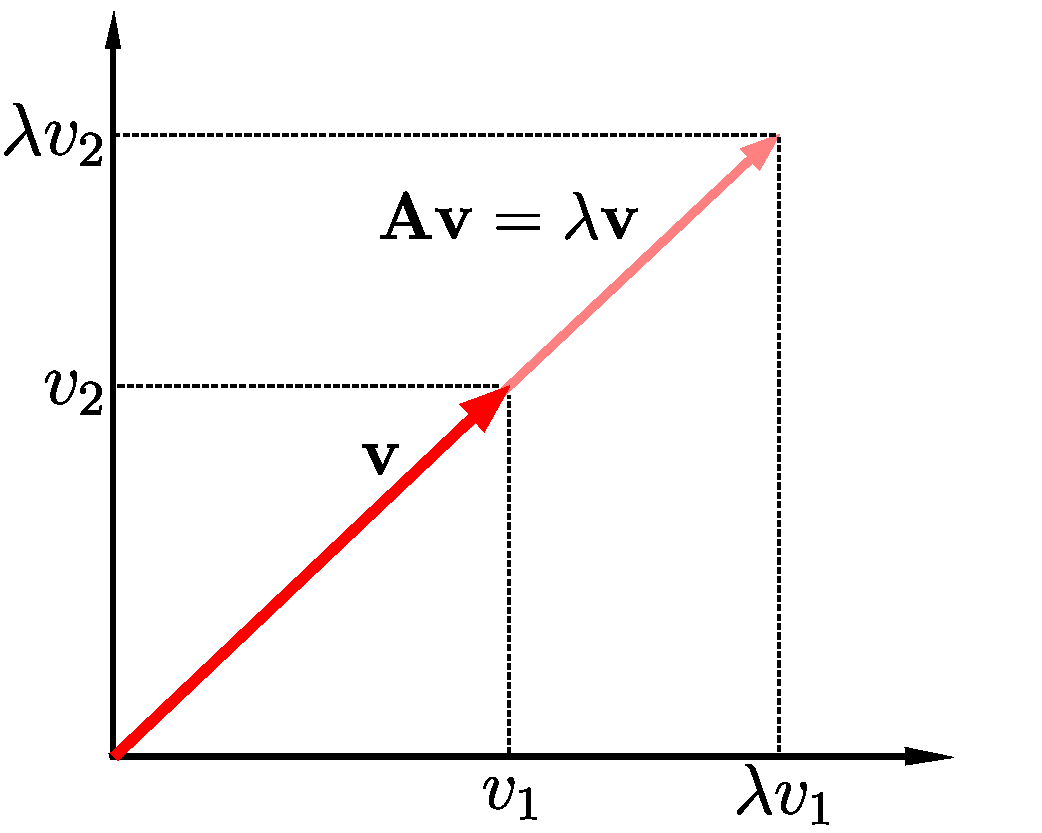
\includegraphics[width=0.5\textwidth]{figs/linear-algebra/eigenvalue_equation.pdf}
    \caption{Visualization of the eigenvalue equation $ \mathbf{A}\mathbf{v} = \lambda \mathbf{v} $, where $\mathbf{v} = (v_1, v_2)$.}
    \label{fig:eigenvalue-equation}
\end{figure}

Formally, for a matrix $\mathbf{A} \in \mathbb{R}^{n\times n}$, a non-zero vector $\mathbf{v}$ is an eigenvector if it satisfies the equation:
$$ \mathbf{A}\mathbf{v} = \lambda \mathbf{v} $$
The scalar $\lambda$ is the corresponding \textbf{eigenvalue}, which represents the scaling factor. An $n \times n$ matrix has at most $n$ distinct eigenvalues.

\begin{warningBox}
    \textbf{Warning:} An eigenvector is not unique. If $\mathbf{v}$ is an eigenvector, then so is any scalar multiple $c\mathbf{v}$ for $c \neq 0$. They both correspond to the same eigenvalue and define the same invariant direction.
\end{warningBox}

The concept is very important for understanding iterative methods. For example, look at the Jacobi iteration error propagation (which we will encounter shortly), $e_{t+1} = \mathbf{S}e_t$, which implies $e_t = \mathbf{S}^t e_0$. Eigenvalues and eigenvectors tell us what happens to a vector when it's multiplied by the same matrix repeatedly.

\subsection{Finding Eigenvalues and Eigenvectors}

To find eigenvalues, we rearrange the defining equation:
$$ \mathbf{A}\mathbf{v} - \lambda \mathbf{v} = 0 \implies (\mathbf{A} - \lambda \mathbf{I})\mathbf{v} = 0 $$
For this equation to have a non-trivial solution for $\mathbf{v}$ (i.e., $\mathbf{v} \neq 0$), the matrix $(\mathbf{A} - \lambda \mathbf{I})$ must be singular. This means its determinant must be zero.
$$ \det(\mathbf{A} - \lambda \mathbf{I}) = 0 $$
This equation defines the \textbf{characteristic polynomial} of $\mathbf{A}$, an $n$-degree polynomial in $\lambda$. Its $n$ roots (which may be real or complex and are counted with algebraic multiplicity) are the eigenvalues of $\mathbf{A}$.

Solving the characteristic polynomial is practical for small, textbook examples. However, this method is generally ill-conditioned and not recommended for numerical work with larger matrices; robust iterative algorithms (e.g., QR/Schur) are used in practice.

Once an eigenvalue $\lambda_i$ is found, the corresponding eigenvector(s) $\mathbf{v}_i$ are found by solving the linear system $(\mathbf{A} - \lambda_i \mathbf{I})\mathbf{v}_i = 0$, which is equivalent to finding the null space of $(\mathbf{A} - \lambda_i \mathbf{I})$.

\begin{exampleBox}
    \textbf{Example (finding eigenvalues and eigenvectors):}
    Let $\mathbf{A} = \begin{bmatrix} -2 & 1 \\ 1 & -2 \end{bmatrix}$.

    \textbf{1. Find Eigenvalues:}
    Solve $\det(\mathbf{A} - \lambda \mathbf{I}) = 0$:
    $$ \det \begin{bmatrix} -2-\lambda & 1 \\ 1 & -2-\lambda \end{bmatrix} = (-2-\lambda)^2 - 1 = \lambda^2 + 4\lambda + 3 = 0 $$
    Factoring gives $(\lambda+3)(\lambda+1)=0$. The eigenvalues are $\lambda_1 = -3$ and $\lambda_2 = -1$.

    \textbf{2. Find Eigenvectors:}
    For $\lambda_1 = -3$, we solve $(\mathbf{A} - (-3)\mathbf{I})\mathbf{v}_1 = 0$:
    $$ \begin{bmatrix} 1 & 1 \\ 1 & 1 \end{bmatrix} \begin{bmatrix} v_1 \\ v_2 \end{bmatrix} = \begin{bmatrix} 0 \\ 0 \end{bmatrix} \implies v_1 + v_2 = 0 $$
    An eigenvector is $\mathbf{v}_1 = \begin{bmatrix} 1 \\ -1 \end{bmatrix}$.

    For $\lambda_2 = -1$, we solve $(\mathbf{A} - (-1)\mathbf{I})\mathbf{v}_2 = 0$:
    $$ \begin{bmatrix} -1 & 1 \\ 1 & -1 \end{bmatrix} \begin{bmatrix} v_1 \\ v_2 \end{bmatrix} = \begin{bmatrix} 0 \\ 0 \end{bmatrix} \implies -v_1 + v_2 = 0 $$
    An eigenvector is $\mathbf{v}_2 = \begin{bmatrix} 1 \\ 1 \end{bmatrix}$.
\end{exampleBox}

\subsection{Multiplicity and Diagonalizability}

The number of times an eigenvalue appears as a root of the characteristic polynomial is its \textbf{algebraic multiplicity}. The number of linearly independent eigenvectors for that eigenvalue is its \textbf{geometric multiplicity}. For any eigenvalue, $1 \le \text{geometric multiplicity} \le \text{algebraic multiplicity}$. A matrix is called \textbf{defective} if for some eigenvalue its geometric multiplicity is less than its algebraic multiplicity; equivalently, it does not have \(n\) linearly independent eigenvectors. A matrix with a ``complete set'' of eigenvectors (geometric = algebraic multiplicity for all eigenvalues) is \textbf{diagonalizable}.

\subsection{Eigendecomposition}
If an $n \times n$ matrix $\mathbf{A}$ is diagonalizable, it has $n$ linearly independent eigenvectors $\{\mathbf{v}_1, \dots, \mathbf{v}_n\}$. We can bundle these into a matrix $\mathbf{W} = [\mathbf{v}_1 | \dots | \mathbf{v}_n]$ and the corresponding eigenvalues into a diagonal matrix $\mathbf{\Lambda}$. The eigenvalue equation for all eigenvectors can be written compactly as:
$$ \mathbf{A}\mathbf{W} = \mathbf{W}\mathbf{\Lambda} $$
This leads to the \textbf{eigendecomposition} of $\mathbf{A}$:
$$ \mathbf{A} = \mathbf{W} \mathbf{\Lambda} \mathbf{W}^{-1} \quad \text{and} \quad \mathbf{\Lambda} = \mathbf{W}^{-1} \mathbf{A} \mathbf{W} $$
This decomposition reveals the fundamental behavior of $\mathbf{A}$ as a simple scaling along the eigenvector axes.

\begin{theoremBox}
    \textbf{Properties and Special Cases} \\
    For a matrix $\mathbf{A} \in \mathbb{R}^{n \times n}$ with eigenvalues $\lambda_1, \dots, \lambda_n$:
    \begin{itemize}
        \item The determinant is the product of its eigenvalues: $\det(\mathbf{A}) = \prod_{i=1}^n \lambda_i$.
        \item The trace is the sum of its eigenvalues: $\operatorname{tr}(\mathbf{A}) = \sum_{i=1}^n \lambda_i$.
        \item The eigenvalues of a triangular matrix are its diagonal entries.
    \end{itemize}
    If $\mathbf{A}$ is a real symmetric matrix ($\mathbf{A} = \mathbf{A}^T$):
    \begin{itemize}
        \item It is always diagonalizable and has a complete set of orthonormal eigenvectors.
        \item All its eigenvalues are real.
        \item Its eigendecomposition is $\mathbf{A} = \mathbf{W} \mathbf{\Lambda} \mathbf{W}^T$, where $\mathbf{W}$ is an orthogonal matrix ($\mathbf{W}^{-1} = \mathbf{W}^T$).
        \item If $\mathbf{A}$ is positive definite, all its eigenvalues are positive ($\lambda_i > 0$).
    \end{itemize}
\end{theoremBox}


\section{Numerical Solution of Linear Systems: Iterative Methods}
\label{sec:num_sol_linear_iterative}
Iterative methods attempt to solve linear systems ($\mathbf{A}\mathbf{x} = \mathbf{b}$) by generating a sequence of improving approximate solutions. They do not require Gaussian elimination and generally scale better for large systems. However, even with infinite precision, iterative methods can only obtain an approximate solution in a finite number of steps\footnote{Actually, some iterative methods, like CG on SPD, are finite-termination in exact arithmetic, but we aren't going to cover that in this course.}. We cover Jacobi and Gauss-Seidel iteration, two of the most common iterative methods, in this course. But one more extremely popular method deserves at least a mention: the conjugate gradient method.\footnote{A good resource for this is Prof. Jonathan Shewchuk's guide \textit{An Introduction to the Conjugate Gradient Method Without the Agonizing Pain}.\autocite{shewchuk1994}}

\subsection{Jacobi Iteration}
Jacobi iteration is an iterative method for solving linear systems. Let's build some intuition for this method before giving the matrix form of the update formula. Suppose we have the linear system
\begin{align*}
    a_{11}x_1 + a_{12}x_2 + \dots + a_{1n} & = b_1 \\
    a_{21}x_1 + a_{22}x_2 + \dots + a_{2n} & = b_2 \\
    \vdots & \\
    a_{n1}x_1 + a_{n2}x_2 + \dots + a_{nn} & = b_n
\end{align*}
and some initial approximation/guess for the solution, $ x_1^{(0)}, x_2^{(0)}, \dots, x_n^{(0)} $. How can we improve this guess? Well, rewriting the $i$-th equation in terms of the other variables, we have
\begin{equation*}
    x_i = \frac{1}{a_{ii}} \left( b_i - \sum_{j \neq i} a_{ij}x_j \right)
\end{equation*}
If this equation is satisfied, then the $i$-th equation of the linear system is also satisfied. So, to improve our guess for $x_i$, we can use the current values of the other variables to estimate the value of $x_i$. After doing this for each variable (which we can do in parallel---we only update the values of the variables \textit{after} we have computed the new values for all of them), we have a new approximation for the solution. We can then repeat this process until the solution converges (assuming that it does---more on this later). This is the main idea behind Jacobi iteration.
\begin{warningBox}
    \textbf{Warning}: One might be tempted to think that after one iteration, we have the exact solution for $x_i$ (after all, we solve each $i$-th equation exactly, right?). You should make sure you completely understand why this is not the case before moving on. The Jacobi method is an iterative method, meaning that we must repeat this process multiple times to get a better approximation for the solution.
\end{warningBox}

\textbf{Matrix Formulation}\quad Now, let's put this in matrix form, which is much more convenient for computer implementation. We decompose the coefficient matrix $\mathbf{A}$ into its diagonal component $\mathbf{D}$ and the remainder $\mathbf{R}$, such that $\mathbf{A} = \mathbf{D} + \mathbf{R}$. Here, $\mathbf{D}$ consists of the diagonal elements of $\mathbf{A}$, and $\mathbf{R}$ contains the off-diagonal elements. Thus, the linear system can be rewritten as
\begin{equation*}
    \left( \mathbf{D} + \mathbf{R} \right)\mathbf{x} = \mathbf{b}
    \implies
    \mathbf{D}\mathbf{x} = -\mathbf{R}\mathbf{x} + \mathbf{b}
\end{equation*}
This defines the iterative map
\begin{equation*}
    \mathbf{D}\mathbf{x}^{(i+1)} = -\mathbf{R}\mathbf{x}^{(i)} + \mathbf{b}
\end{equation*}
Assuming that $\mathbf{D}$ is nonsingular, this can be equivalently written as
\begin{equation*}
    \mathbf{x}^{(i+1)} = -\mathbf{D}^{-1}(\mathbf{R}\mathbf{x}^{(i)} - \mathbf{b})
\end{equation*}
This formulation allows us to compute the next approximation $\mathbf{x}^{(i+1)}$ based on the current approximation $\mathbf{x}^{(i)}$. Note how this is the \textit{exact} same formula as the one we derived earlier for the $i$-th variable in the linear system, just written in matrix form so that we can update all variables simultaneously!

As a quick note on notation, many sources commonly split the matrix $\mathbf{A}$ into the sum of a lower triangular matrix $\mathbf{L}$, a diagonal matrix $\mathbf{D}$, and an upper triangular matrix $\mathbf{U}$ (i.e., $\mathbf{A} = \mathbf{L} + \mathbf{D} + \mathbf{U}$). The Jacobi method is then written as
\begin{equation*}
    \mathbf{x}^{(i+1)} = -\mathbf{D}^{-1}(\mathbf{L} + \mathbf{U})\mathbf{x}^{(i)} + \mathbf{D}^{-1}\mathbf{b}
\end{equation*}
This is mathematically equivalent to the formulation we have presented here; don't be confused if you see this alternate notation.

\textbf{Computational Complexity}\quad Each iteration of the Jacobi method involves diagonal matrix inversion, matrix-vector multiplications, and vector updates. Specifically, computing $\mathbf{R}\mathbf{x}^{(i)}$ requires $O(n^2)$ operations for an $n \times n$ matrix $\mathbf{A}$, and the subsequent vector operations also scale quadratically. Inverting a diagonal matrix is trivial and requires only $n$ divisions. Therefore, the computational complexity of each Jacobi iteration is $O(n^2)$.

\subsection{Convergence of Jacobi Iteration}
We have seen that we can generate a sequence of improving approximations $\{\mathbf{x}^{(i)}\}$ to the solution of a linear system using the Jacobi method. But how do we know that this sequence converges at all, and if it converges, that it converges to the true solution $\mathbf{x}^\star$? Convergence is not generally guaranteed for iterative methods, let alone convergence to the true solution.

\textbf{Convergence to the Correct Solution}\quad We claim that if the Jacobi sequence $\{\mathbf{x}^{(i)}\}$ converges, it indeed converges to the correct solution. To see this, we take the limit on both sides of the iterative equation:
\begin{align*}
    \lim_{i \to \infty} \mathbf{x}^{(i+1)} & = \lim_{i \to \infty} -\mathbf{D}^{-1}(\mathbf{R}\mathbf{x}^{(i)} - \mathbf{b}) \\
    \mathbf{x}^\star &= -\mathbf{D}^{-1}(\mathbf{R}\mathbf{x}^\star - \mathbf{b})
\end{align*}
Rearranging terms gives
\begin{equation*}
    \mathbf{D}\mathbf{x}^\star = -\mathbf{R}\mathbf{x}^\star + \mathbf{b} 
    \quad \implies \quad 
    \mathbf{A}\mathbf{x}^\star = \mathbf{b}
\end{equation*}
Thus, the limit $\mathbf{x}^\star$ satisfies the original system, so convergence implies correctness.

\textbf{Conditions for Convergence}\quad So if we converge, we converge to the correct solution. But how do we know if we converge at all? Let's derive the conditions for convergence. We consider the exact solution satisfying
\begin{equation*}
    \mathbf{A x}^\star = \mathbf{b} \iff \mathbf{x}^\star = -\mathbf{D}^{-1}\left(\mathbf{R}\mathbf{x}^\star - \mathbf{b}\right)
\end{equation*}
which means that the error at the $(i+1)$-th iteration is given by (note: the symbol $\mydef$ means ``defined as'')
\begin{align*}
    \mathbf{e}^{(i+1)} \mydef \mathbf{x}^{(i+1)} - \mathbf{x}^* &= -\mathbf{D}^{-1}\mathbf{R}\left(\mathbf{x}^{(i)} - \mathbf{x}^\star\right) \\
    &= -\mathbf{D}^{-1}\mathbf{R}\mathbf{e}^{(i)}
\end{align*}
Notice how this equation is set up; the error at the $(i+1)$-th iteration is a scaled version of the error at the preceding iteration. So if our initial guess is $\mathbf{x}^{(0)}$, we can keep applying this formula up to the $i$-th iteration to get
\begin{equation*}
    \mathbf{e}^{(i)} = \left( -\mathbf{D}^{-1}\mathbf{R} \right)^i \mathbf{e}^{(0)}
\end{equation*}
This is a very powerful result. To see why, let's use the eigendecomposition\footnote{If the matrix is not diagonalizable, analogous bounds via Jordan form or induced norms still give that $\rho<1$ is necessary and sufficient for linear convergence.} of $-\mathbf{D}^{-1}\mathbf{R}$ to write
\begin{align*}
    \mathbf{e}^{(i)} &=  \left( -\mathbf{D}^{-1}\mathbf{R} \right)^i \mathbf{e}^{(0)} & \\
    &= \left(\mathbf{W} \boldsymbol{\Lambda} \mathbf{W}^{-1}\right)^i \mathbf{e}^{(0)} &\text{(eigendecomposition)} \\
    &= \left(\mathbf{W} \boldsymbol{\Lambda} \mathbf{W}^{-1}\right)\left(\mathbf{W} \boldsymbol{\Lambda} \mathbf{W}^{-1}\right)\cdots\left(\mathbf{W} \boldsymbol{\Lambda} \mathbf{W}^{-1}\right) \mathbf{e}^{(0)} &\text{(expand power)}\\
    &= \mathbf{W} \boldsymbol{\Lambda} \left(\mathbf{W}^{-1}\mathbf{W}\right)\cdots \boldsymbol{\Lambda} \left(\mathbf{W}^{-1}\mathbf{W}\right) \boldsymbol{\Lambda} \mathbf{W}^{-1}\mathbf{e}^{(0)} &\text{(exploit associativity)} \\
    &= \mathbf{W} \boldsymbol{\Lambda} \left(\mathbf{I}\right)\cdots \boldsymbol{\Lambda} \left(\mathbf{I}\right) \boldsymbol{\Lambda} \mathbf{W}^{-1} \mathbf{e}^{(0)} &\text{(definition of inverse)} \\
    &= \mathbf{W} \boldsymbol{\Lambda}^i \mathbf{W}^{-1} \mathbf{e}^{(0)} &
\end{align*}
Thus, if any of the eigenvalues of $-\mathbf{D}^{-1}\mathbf{R}$ have magnitude greater than 1, the error will grow with $i$, and the Jacobi method will not converge. On the other hand, if all the eigenvalues have magnitude less than 1, the error will decay with $i$, and the Jacobi method will converge. And if any eigenvalues have magnitude equal to 1, the error will either remain constant or oscillate. In linear algebraic terms, this is captured by the notion of the \textbf{spectral radius} $\rho$ of $-\mathbf{D}^{-1}\mathbf{R}$, which is the maximum magnitude of the eigenvalues of $-\mathbf{D}^{-1}\mathbf{R}$. Indeed, since we also know that convergence implies correctness, we have that
\begin{equation*}
    \rho(-\mathbf{D}^{-1}\mathbf{R}) < 1 \implies \|\mathbf{x}^{(i)} - \mathbf{x}^\star\|_p \to 0 \quad \text{as } i \to \infty
\end{equation*}
or, in words, the Jacobi method converges to the correct solution if the spectral radius of $-\mathbf{D}^{-1}\mathbf{R}$ is less than 1.

The most natural question to ask is when the spectral radius of $-\mathbf{D}^{-1}\mathbf{R}$ is less than 1. The answer is that this is true if $\mathbf{A}$ (recall that $\mathbf{A} = \mathbf{D} + \mathbf{R}$) is diagonally dominant. A matrix is diagonally dominant if for every row $i$, the diagonal element $a_{ii}$ is greater in magnitude than the sum of the magnitudes of the off-diagonal elements in that row. In mathematical terms, this is written as
\begin{equation*}
    |a_{ii}| > \sum_{j \neq i} |a_{ij}|
\end{equation*}

\textbf{Rate of Convergence}\quad The speed at which the Jacobi iteration converges to the solution $\mathbf{x}^\star$ is characterized by the spectral radius $\alpha = \rho(-\mathbf{D}^{-1}\mathbf{R})$. The error after $i$ iterations can be approximated as
\begin{equation*}
    \|\mathbf{x}^{(i)} - \mathbf{x}^\star\|_p \approx O(\alpha^i) \|\mathbf{x}_0 - \mathbf{x}^\star\|_p
\end{equation*}
Here, $\alpha$ is referred to as the \textbf{rate of convergence}. To achieve a desired accuracy $\epsilon$, the number of iterations required satisfies
\begin{equation*}
    \frac{\|\mathbf{x}^{(i)} - \mathbf{x}^\star\|_p}{\|\mathbf{x}_0 - \mathbf{x}^\star\|_p} \leq \epsilon 
    \quad\implies\quad 
    i \geq \frac{\log(\epsilon)}{\log(\alpha)}
\end{equation*}
A smaller $\alpha$ indicates faster convergence. However, the Jacobi method can be relatively slow compared to other iterative methods like Gauss-Seidel or successive over-relaxation (SOR, not covered in this course), especially when $\alpha$ is close to 1.

\subsection{Gauss-Seidel Iteration}
Gauss-Seidel iteration is another iterative method for solving linear systems, similar to the Jacobi method but often exhibiting faster convergence. Like Jacobi iteration, it builds a sequence of approximations to the solution, but it uses the most recently updated values within each iteration to enhance convergence speed.

Consider the same linear system as before:
\begin{align*}
    a_{11}x_1 + a_{12}x_2 + \dots + a_{1n} & = b_1 \\
    a_{21}x_1 + a_{22}x_2 + \dots + a_{2n} & = b_2 \\
    \vdots & \\
    a_{n1}x_1 + a_{n2}x_2 + \dots + a_{nn} & = b_n
\end{align*}
and an initial guess for the solution, $ x_1^{(0)}, x_2^{(0)}, \dots, x_n^{(0)} $. To improve this guess, Gauss-Seidel iteration updates each variable sequentially, immediately using the latest available values. Specifically, the update rule for the $i$-th variable is
\begin{equation*}
    x_i^{(k+1)} = \frac{1}{a_{ii}} \left( b_i - \sum_{j < i} a_{ij}x_j^{(k+1)} - \sum_{j > i} a_{ij}x_j^{(k)} \right)
\end{equation*}
for $ i = 1, 2, \dots, n $, where $ k $ denotes the current iteration. This means that when computing $ x_i^{(k+1)} $, the most recent values $ x_1^{(k+1)}, \dots, x_{i-1}^{(k+1)} $ are already updated, whereas $ x_{i+1}^{(k)}, \dots, x_n^{(k)} $ remain from the previous iteration. You should convince yourself that this update rule makes sense and compare it to the Jacobi update rule before proceeding.

\begin{warningBox}
    \textbf{Warning}: Unlike the Jacobi method, Gauss-Seidel updates variables sequentially and relies on the latest available estimates within the same iteration. This sequential dependency can lead to faster convergence but may complicate parallel implementations.
\end{warningBox}

\textbf{Matrix Formulation}\quad To express Gauss-Seidel iteration in matrix form, we decompose the coefficient matrix $\mathbf{A}$ into its lower triangular component $\mathbf{L}$, diagonal component $\mathbf{D}$, and upper triangular component $\mathbf{U}$, such that
\begin{equation*}
    \mathbf{A} = \mathbf{L} + \mathbf{D} + \mathbf{U}
\end{equation*}
where $\mathbf{L}$ contains the strictly lower triangular elements of $\mathbf{A}$, $\mathbf{D}$ is the diagonal matrix of $\mathbf{A}$, and $\mathbf{U}$ contains the strictly upper triangular elements of $\mathbf{A}$. The linear system can then be rewritten as
\begin{equation*}
    (\mathbf{D} + \mathbf{L})\mathbf{x} = -\mathbf{U}\mathbf{x} + \mathbf{b}
\end{equation*}
This defines the iterative map for Gauss-Seidel:
\begin{equation*}
    (\mathbf{D} + \mathbf{L})\mathbf{x}^{(k+1)} = -\mathbf{U}\mathbf{x}^{(k)} + \mathbf{b}
\end{equation*}
Assuming $\mathbf{D} + \mathbf{L}$ is nonsingular, we can solve for $\mathbf{x}^{(k+1)}$ to get
\begin{equation*}
    \mathbf{x}^{(k+1)} = -(\mathbf{D} + \mathbf{L})^{-1}\mathbf{U}\mathbf{x}^{(k)} + (\mathbf{D} + \mathbf{L})^{-1}\mathbf{b}
\end{equation*}
This formulation allows for sequential updates of the solution vector, utilizing the latest available estimates within each iteration. This is exactly the same as the update rule we derived earlier, just written in matrix form for convenience.

\textbf{Computational Complexity}\quad Each Gauss-Seidel iteration involves solving a lower triangular system due to the $\mathbf{L} + \mathbf{D}$ term. Luckily, we can do this with forward substitution with $O(n^2)$ operations, so the computational complexity remains similar to Jacobi. That is, it is $O(n^2)$ operations per iteration for an $n \times n$ matrix $\mathbf{A}$.

\subsection{Convergence of Gauss-Seidel Iteration}
As with the Jacobi method, the convergence of Gauss-Seidel iteration is not universally guaranteed. However, under certain conditions, convergence can be assured, and when it does converge, it does so to the correct solution.

\textbf{Convergence to the Correct Solution}\quad Assuming the Gauss-Seidel sequence $\{\mathbf{x}^{(k)}\}$ converges to a limit $\mathbf{x}^\star$, we can take the limit on both sides of the iterative equation:
\begin{align*}
    \lim_{k \to \infty} (\mathbf{D} + \mathbf{L})\mathbf{x}^{(k+1)} &= \lim_{k \to \infty} \left( -\mathbf{U}\mathbf{x}^{(k)} + \mathbf{b} \right) \\
    (\mathbf{D} + \mathbf{L})\mathbf{x}^\star &= -\mathbf{U}\mathbf{x}^\star + \mathbf{b} \\
    \mathbf{A}\mathbf{x}^\star &= \mathbf{b}
\end{align*}
Thus, the limit $\mathbf{x}^\star$ satisfies the original linear system, meaning that convergence implies correctness.

\textbf{Conditions for Convergence}\quad To determine when the Gauss-Seidel method converges, we analyze the error propagation similarly to Jacobi iteration. Let $\mathbf{e}^{(k)} = \mathbf{x}^{(k)} - \mathbf{x}^\star$ denote the error at the $k$-th iteration. The iterative relation for the error becomes
\begin{align*}
    (\mathbf{D} + \mathbf{L})\mathbf{e}^{(k+1)} &= -\mathbf{U}\mathbf{e}^{(k)} \\
    \mathbf{e}^{(k+1)} &= -(\mathbf{D} + \mathbf{L})^{-1}\mathbf{U}\mathbf{e}^{(k)}
\end{align*}
Letting $\mathbf{G} = -(\mathbf{D} + \mathbf{L})^{-1}\mathbf{U}$, we have
\begin{equation*}
    \mathbf{e}^{(k+1)} = \mathbf{G}\mathbf{e}^{(k)}
\end{equation*}
By iterating, the error after $k$ iterations is
\begin{equation*}
    \mathbf{e}^{(k)} = \mathbf{G}^k \mathbf{e}^{(0)}
\end{equation*}
Using the eigendecomposition of $\mathbf{G}$, similar to the Jacobi method, we find that the spectral radius $\rho(\mathbf{G})$ governs convergence:
\begin{equation*}
    \rho(\mathbf{G}) < 1 \implies \|\mathbf{x}^{(k)} - \mathbf{x}^\star\|_p \to 0 \quad \text{as } k \to \infty
\end{equation*}
When is $\rho(\mathbf{G}) < 1$? If the matrix $\mathbf{A}$ is strictly diagonally dominant, i.e.,
\begin{equation*}
    |a_{ii}| > \sum_{j \neq i} |a_{ij}| \quad \forall i
\end{equation*}
then the spectral radius $\rho(\mathbf{G}) < 1$, ensuring convergence of the Gauss-Seidel method. Additionally, if $\mathbf{A}$ is symmetric positive definite, convergence is also guaranteed.

\textbf{Rate of Convergence}\quad The rate at which Gauss-Seidel iteration converges is determined by the spectral radius $\alpha = \rho(\mathbf{G})$. The error after $k$ iterations can be approximated by
\begin{equation*}
    \|\mathbf{x}^{(k)} - \mathbf{x}^\star\|_p \approx O(\alpha^k) \|\mathbf{x}^{(0)} - \mathbf{x}^\star\|_p
\end{equation*}
Since $\alpha < 1$ for convergent systems, a smaller $\alpha$ results in faster convergence. Often, it is empirically true that Gauss-Seidel converges faster than Jacobi because it effectively incorporates more up-to-date information within each iteration. However, like Jacobi, the convergence rate depends on the properties of $\mathbf{A}$, and for systems with a spectral radius close to 1, convergence can still be slow.

\textbf{Comparison with Jacobi Iteration}\quad While both methods are simple and easy to implement, Gauss-Seidel typically outperforms Jacobi in terms of convergence speed due to its sequential update strategy. However, this comes at the cost of reduced parallelizability, as each update depends on the results of the previous ones within the same iteration. In contrast, Jacobi's parallel updates make it more suitable for parallel computing environments despite its slower convergence.

In practice, Gauss-Seidel is preferred over Jacobi when faster convergence is desired and when the system structure permits sequential updates without significant computational overhead. For large-scale systems where parallel computation is essential, Jacobi may still be advantageous despite its slower convergence rate.

\subsection{Condition Number and Convergence Rate}
To understand the impact of the condition number on the convergence rate of iterative methods, we consider the Richardson method, an iterative method defined by the update rule
\begin{equation*}
    \mathbf{x}^{(i+1)} = \mathbf{x}^{(i)} + \omega (\mathbf{b} - \mathbf{A}\mathbf{x}^{(i)})
\end{equation*}
where $\omega$ is a relaxation parameter. The choice of $\omega$ strongly affects the convergence behavior of the method. Assuming that $\mathbf{A}$ is symmetric positive definite, the optimal convergence rate for the Richardson method is achieved with the choice
\begin{equation*}
    \omega_{\text{opt}} = \frac{2}{\lambda_{\min}(\mathbf{A}) + \lambda_{\max}(\mathbf{A})}
\end{equation*}
With this optimal $\omega$, the spectral radius of the iteration matrix $\mathbf{I} - \omega_{\text{opt}} \mathbf{A}$ becomes
\begin{equation*}
    \rho(\mathbf{I} - \omega_{\text{opt}} \mathbf{A}) = \frac{\kappa(\mathbf{A}) - 1}{\kappa(\mathbf{A}) + 1}
\end{equation*}
This expression shows that the spectral radius---and consequently the convergence rate---is directly related to the condition number $\kappa(\mathbf{A})$. Specifically, a smaller $\kappa(\mathbf{A})$ leads to a smaller spectral radius, resulting in faster convergence of the iterative method. Conversely, a large condition number implies that the spectral radius is closer to one, which can significantly slow down convergence.

This relationship (not the literal equation, but the idea we just talked about) between the condition number and the convergence rate is not unique to the Richardson method but holds generally for a wide class of iterative methods, including Jacobi and Gauss-Seidel iterations. Therefore, we should make sure that the coefficient matrix $\mathbf{A}$ is well-conditioned in order to achieve efficiency and reliability of these iterative solvers. If $\kappa(\mathbf{A})$ is large, it may be beneficial to precondition the system to reduce the condition number and improve the convergence rate of the iterative method.

\begin{warningBox}
    \textbf{Warning}: While a lower condition number generally promotes faster convergence, it is important to recognize that not all matrices can be easily preconditioned to achieve a desirable condition number. Additionally, some iterative methods may exhibit different sensitivities to the condition number, so the choice of method should consider both the properties of $\mathbf{A}$ and the specific requirements of the problem at hand.
\end{warningBox}

%%% Local Variables:
%%% mode: LaTeX
%%% TeX-master: "../main"
%%% End:
